\documentclass{beamer}
\usetheme{Gelugor}

\usepackage[utf8]{inputenc}
\usepackage{amsmath}
\usepackage{mathtools}
\usepackage[T1]{fontenc}
\usepackage{lipsum}
%% Use any fonts you like.
\usepackage{helvet}
\usepackage{caption}
\usepackage{graphicx}
\usepackage{animate}
\usepackage{xcolor} % 'svgnames' for 'MistyRose'
\usepackage{multirow}

%comment
\newcommand{\comment}[1]{}

%% Use tikz extention
\usepackage{tikz}
\usetikzlibrary{arrows,shapes,trees}
\definecolor{gold}{rgb}{0.85,0.65,0}

\title{Pengaruh Parameter Meteorologi terhadap Kedalaman Lapisan Campuran (\textit{Mixed Layer Depth}) di Perairan Aceh}
%\subtitle{Click Here to Add Subtitle}
\author{Muh. Nur Hidayat}
\date{\today}
\institute{----\\ 
	Pembimbing 1: Prof. Dr. Ir. Syamsul Rizal \\Pembimbing 2: Prof. Dr. Marwan Ramli, M.Si. \\
	Penguji:  \\ 
	Dr. Said Munzir, S.Si., M.Eng.Sc. \\  Dr. Salmawaty, M.Sc.}


\begin{document}

\begin{frame}[plain,t]
\titlepage

\end{frame}


\section{Daftar Isi}
\begin{frame}
\frametitle{Daftar Isi}
\framesubtitle{Table of Contents}
\begin{itemize}
\item Pendahuluan
\item Tinjauan Pustaka
	\begin{itemize}
	\item Persamaan Gerak Fluida
	\item Persamaan Primitif
	\item Arakawa C-grid
	\item Model Iklim
	\item Kedalaman Lapisan Campuran 
	\end{itemize}
\item Metodologi Penelitian
\item Output Proposal Tesis
\end{itemize}
\end{frame}

\section{Pendahuluan}
\begin{frame}
	\centering
	\begin{figure}[H]
		\centering
		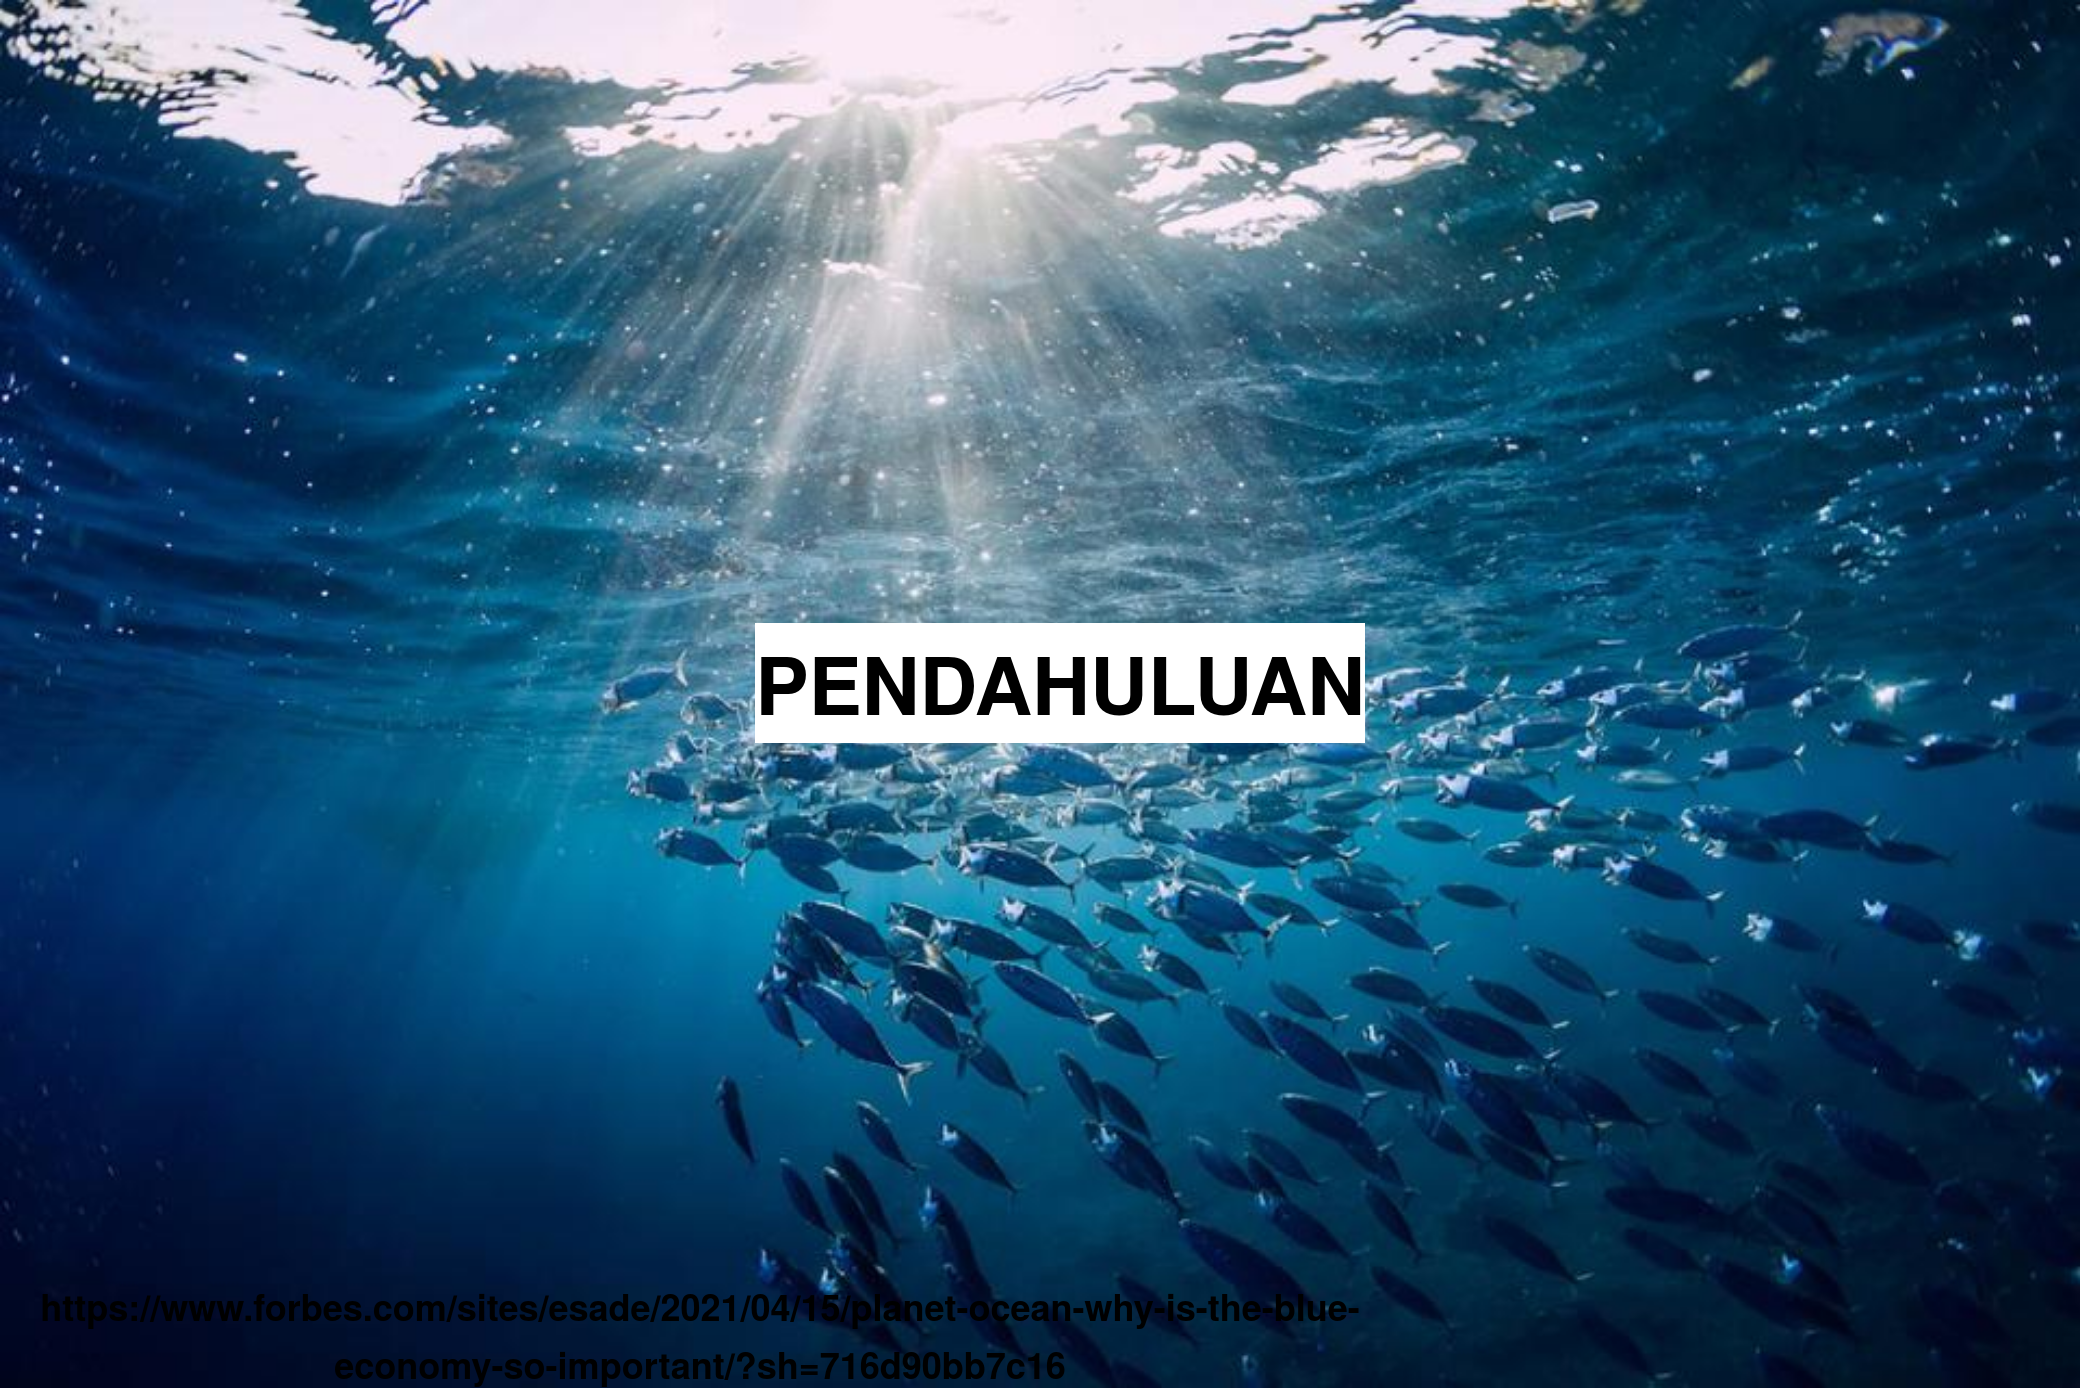
\includegraphics[width=10cm]{Bg_1}
	\end{figure}
\end{frame}
\subsection{Latar Belakang}
\begin{frame}[allowframebreaks]
\frametitle{Latar Belakang}
%	\lipsum[75]
	\begin{figure}[H]
		\centering
		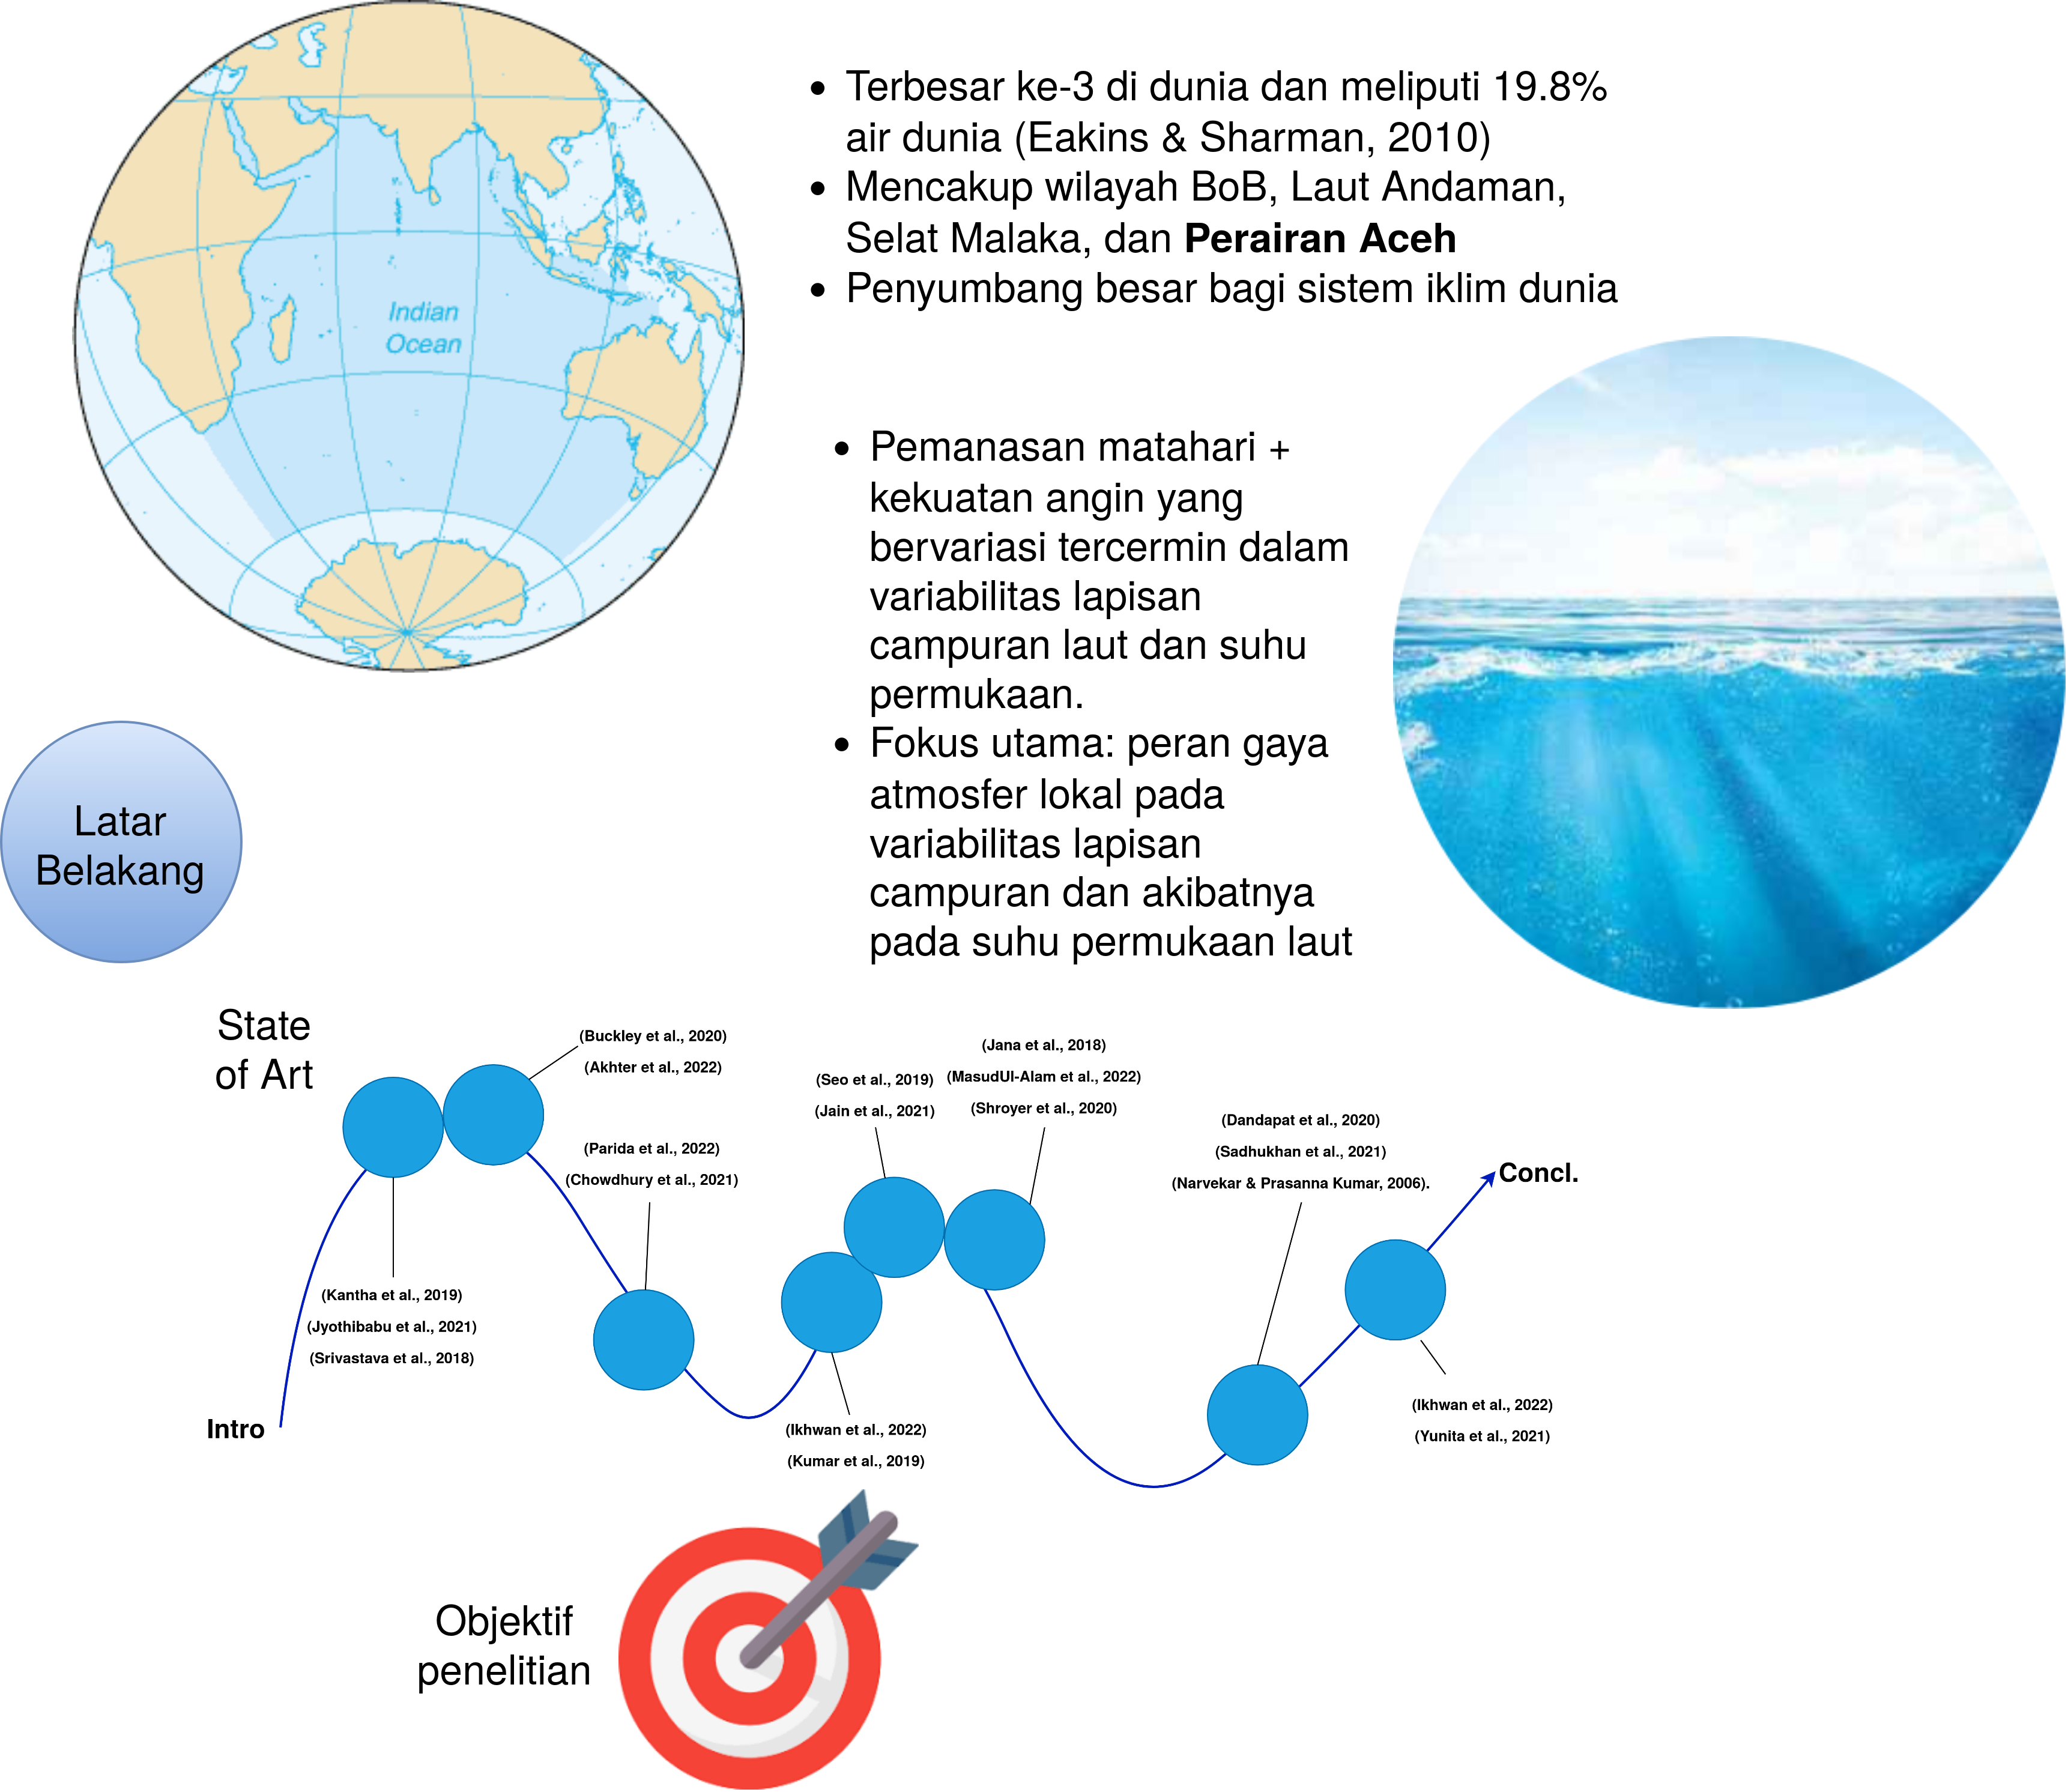
\includegraphics[width=8cm]{intro-0}
	\end{figure}
	\begin{figure}[H]
		\centering
		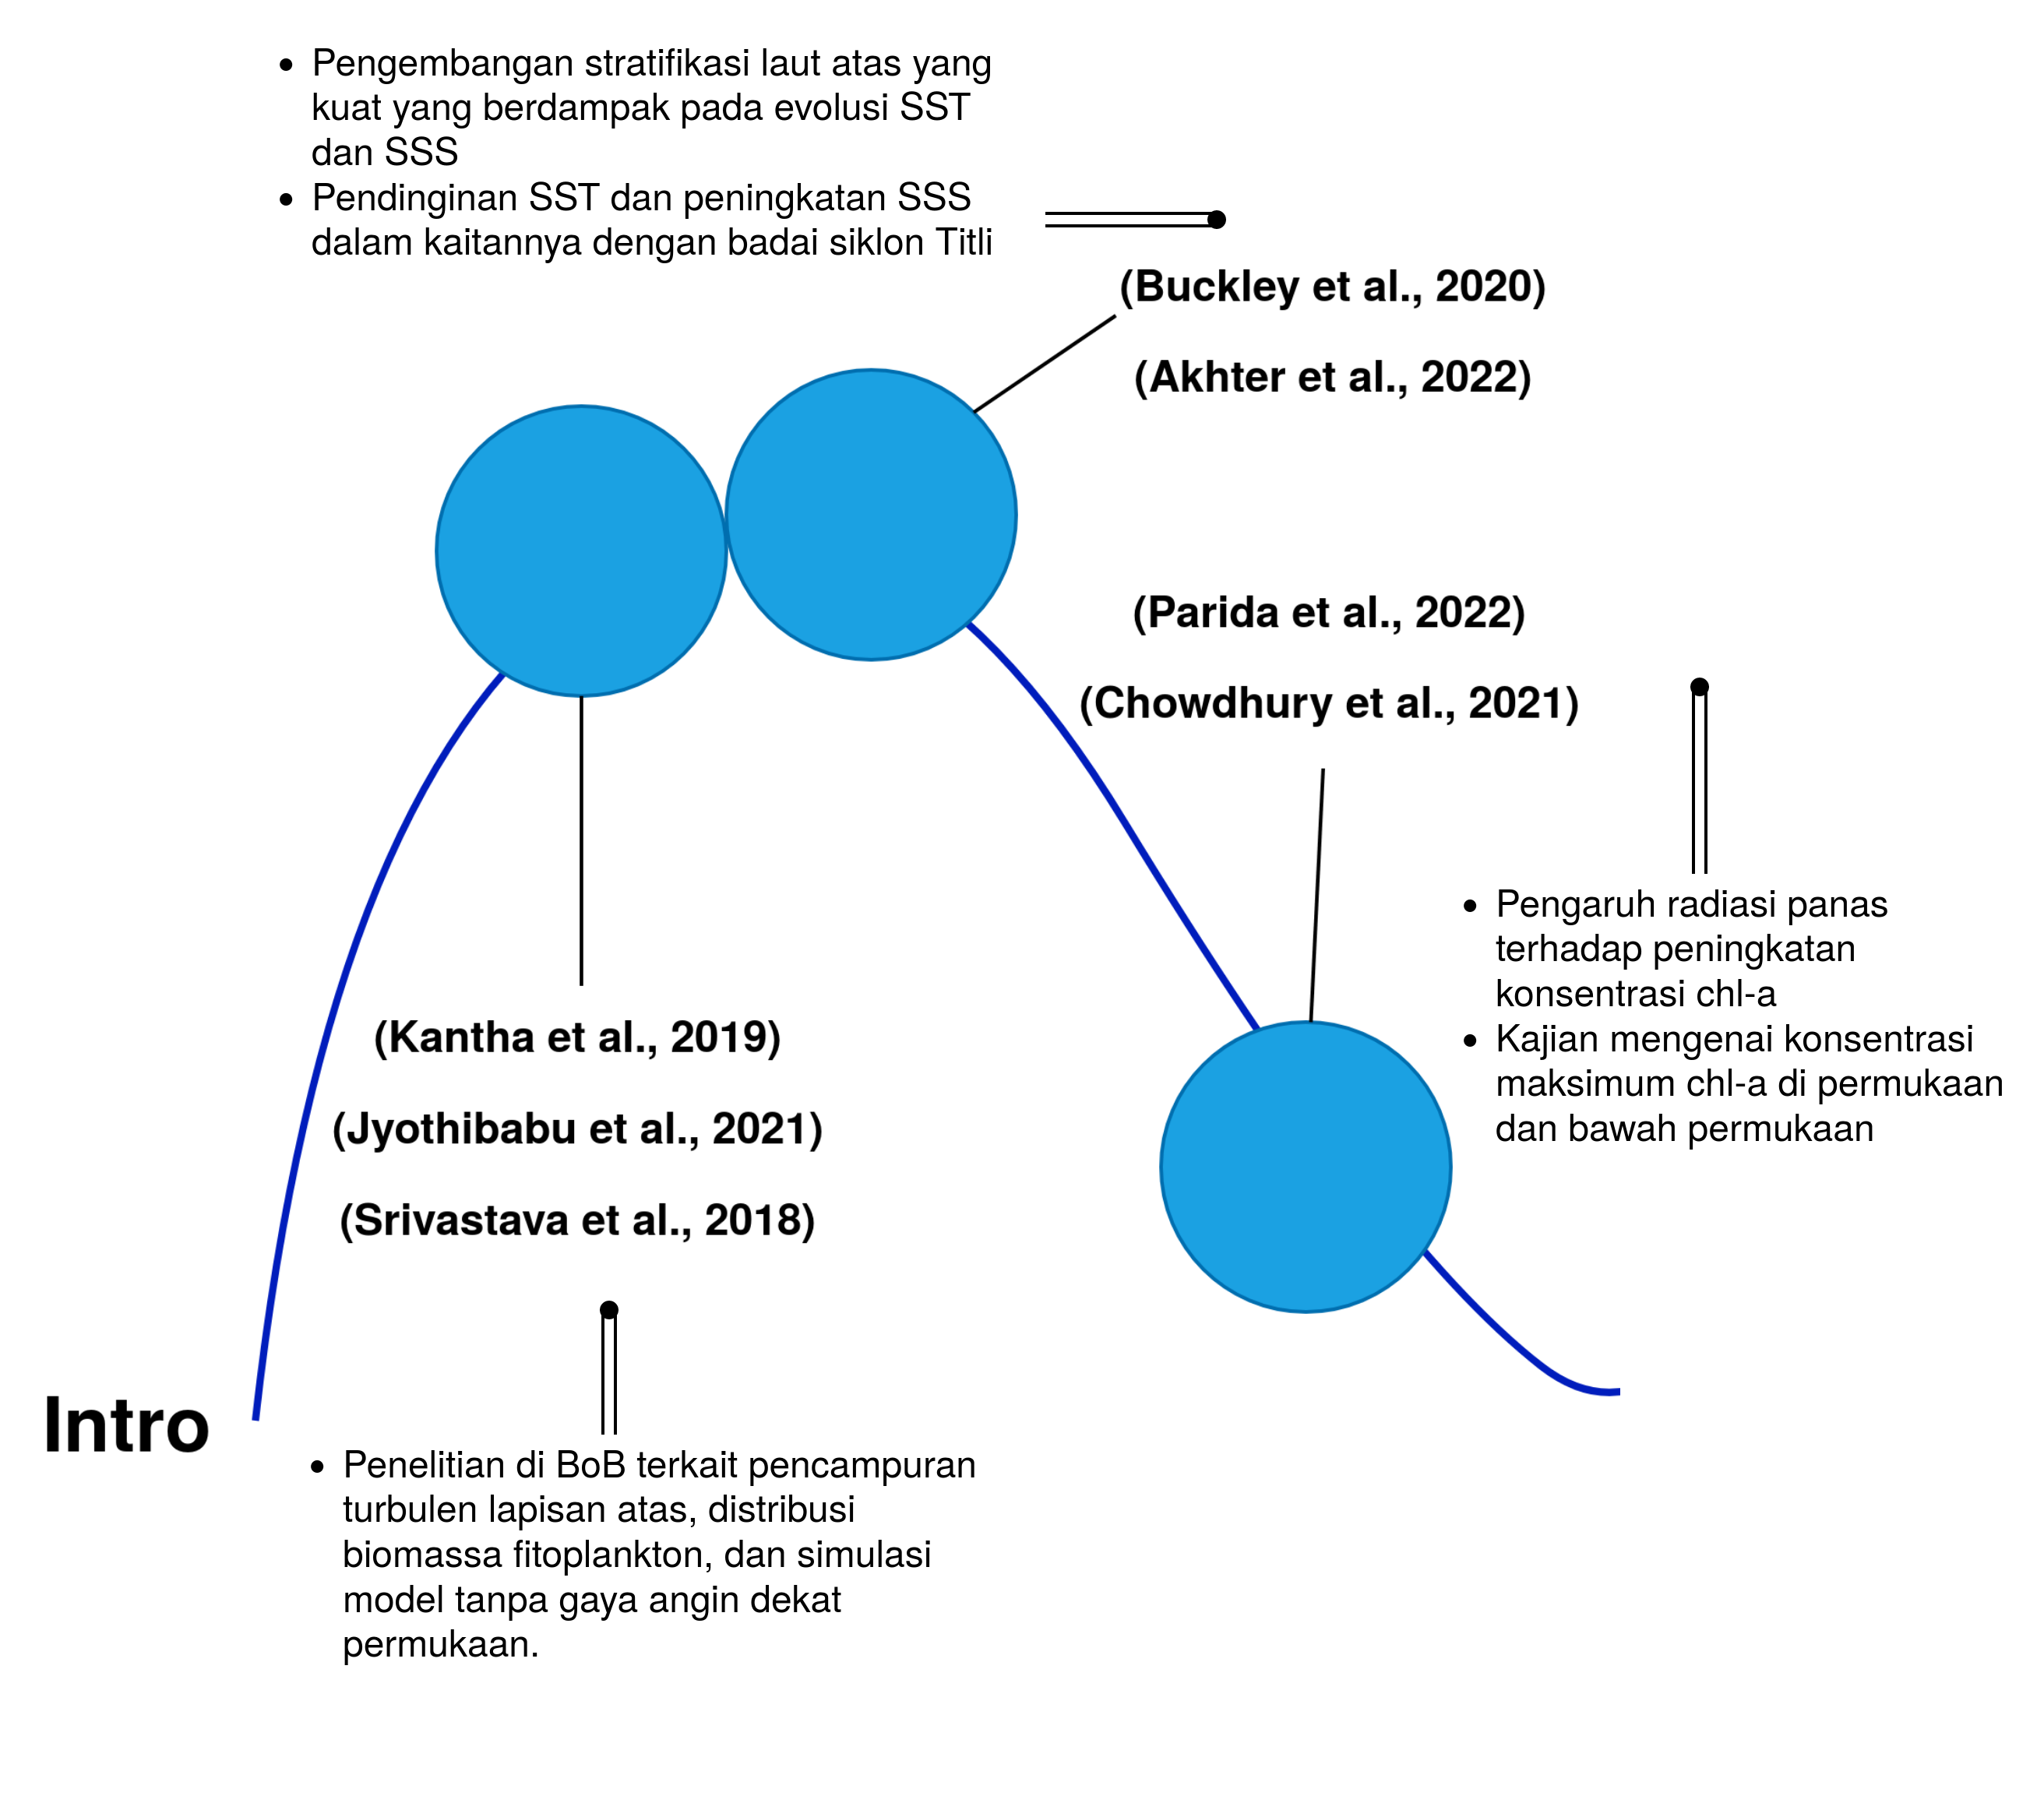
\includegraphics[width=8cm]{intro-1_1}
	\end{figure}
%	\newpage
	\begin{figure}[H]
		\centering
		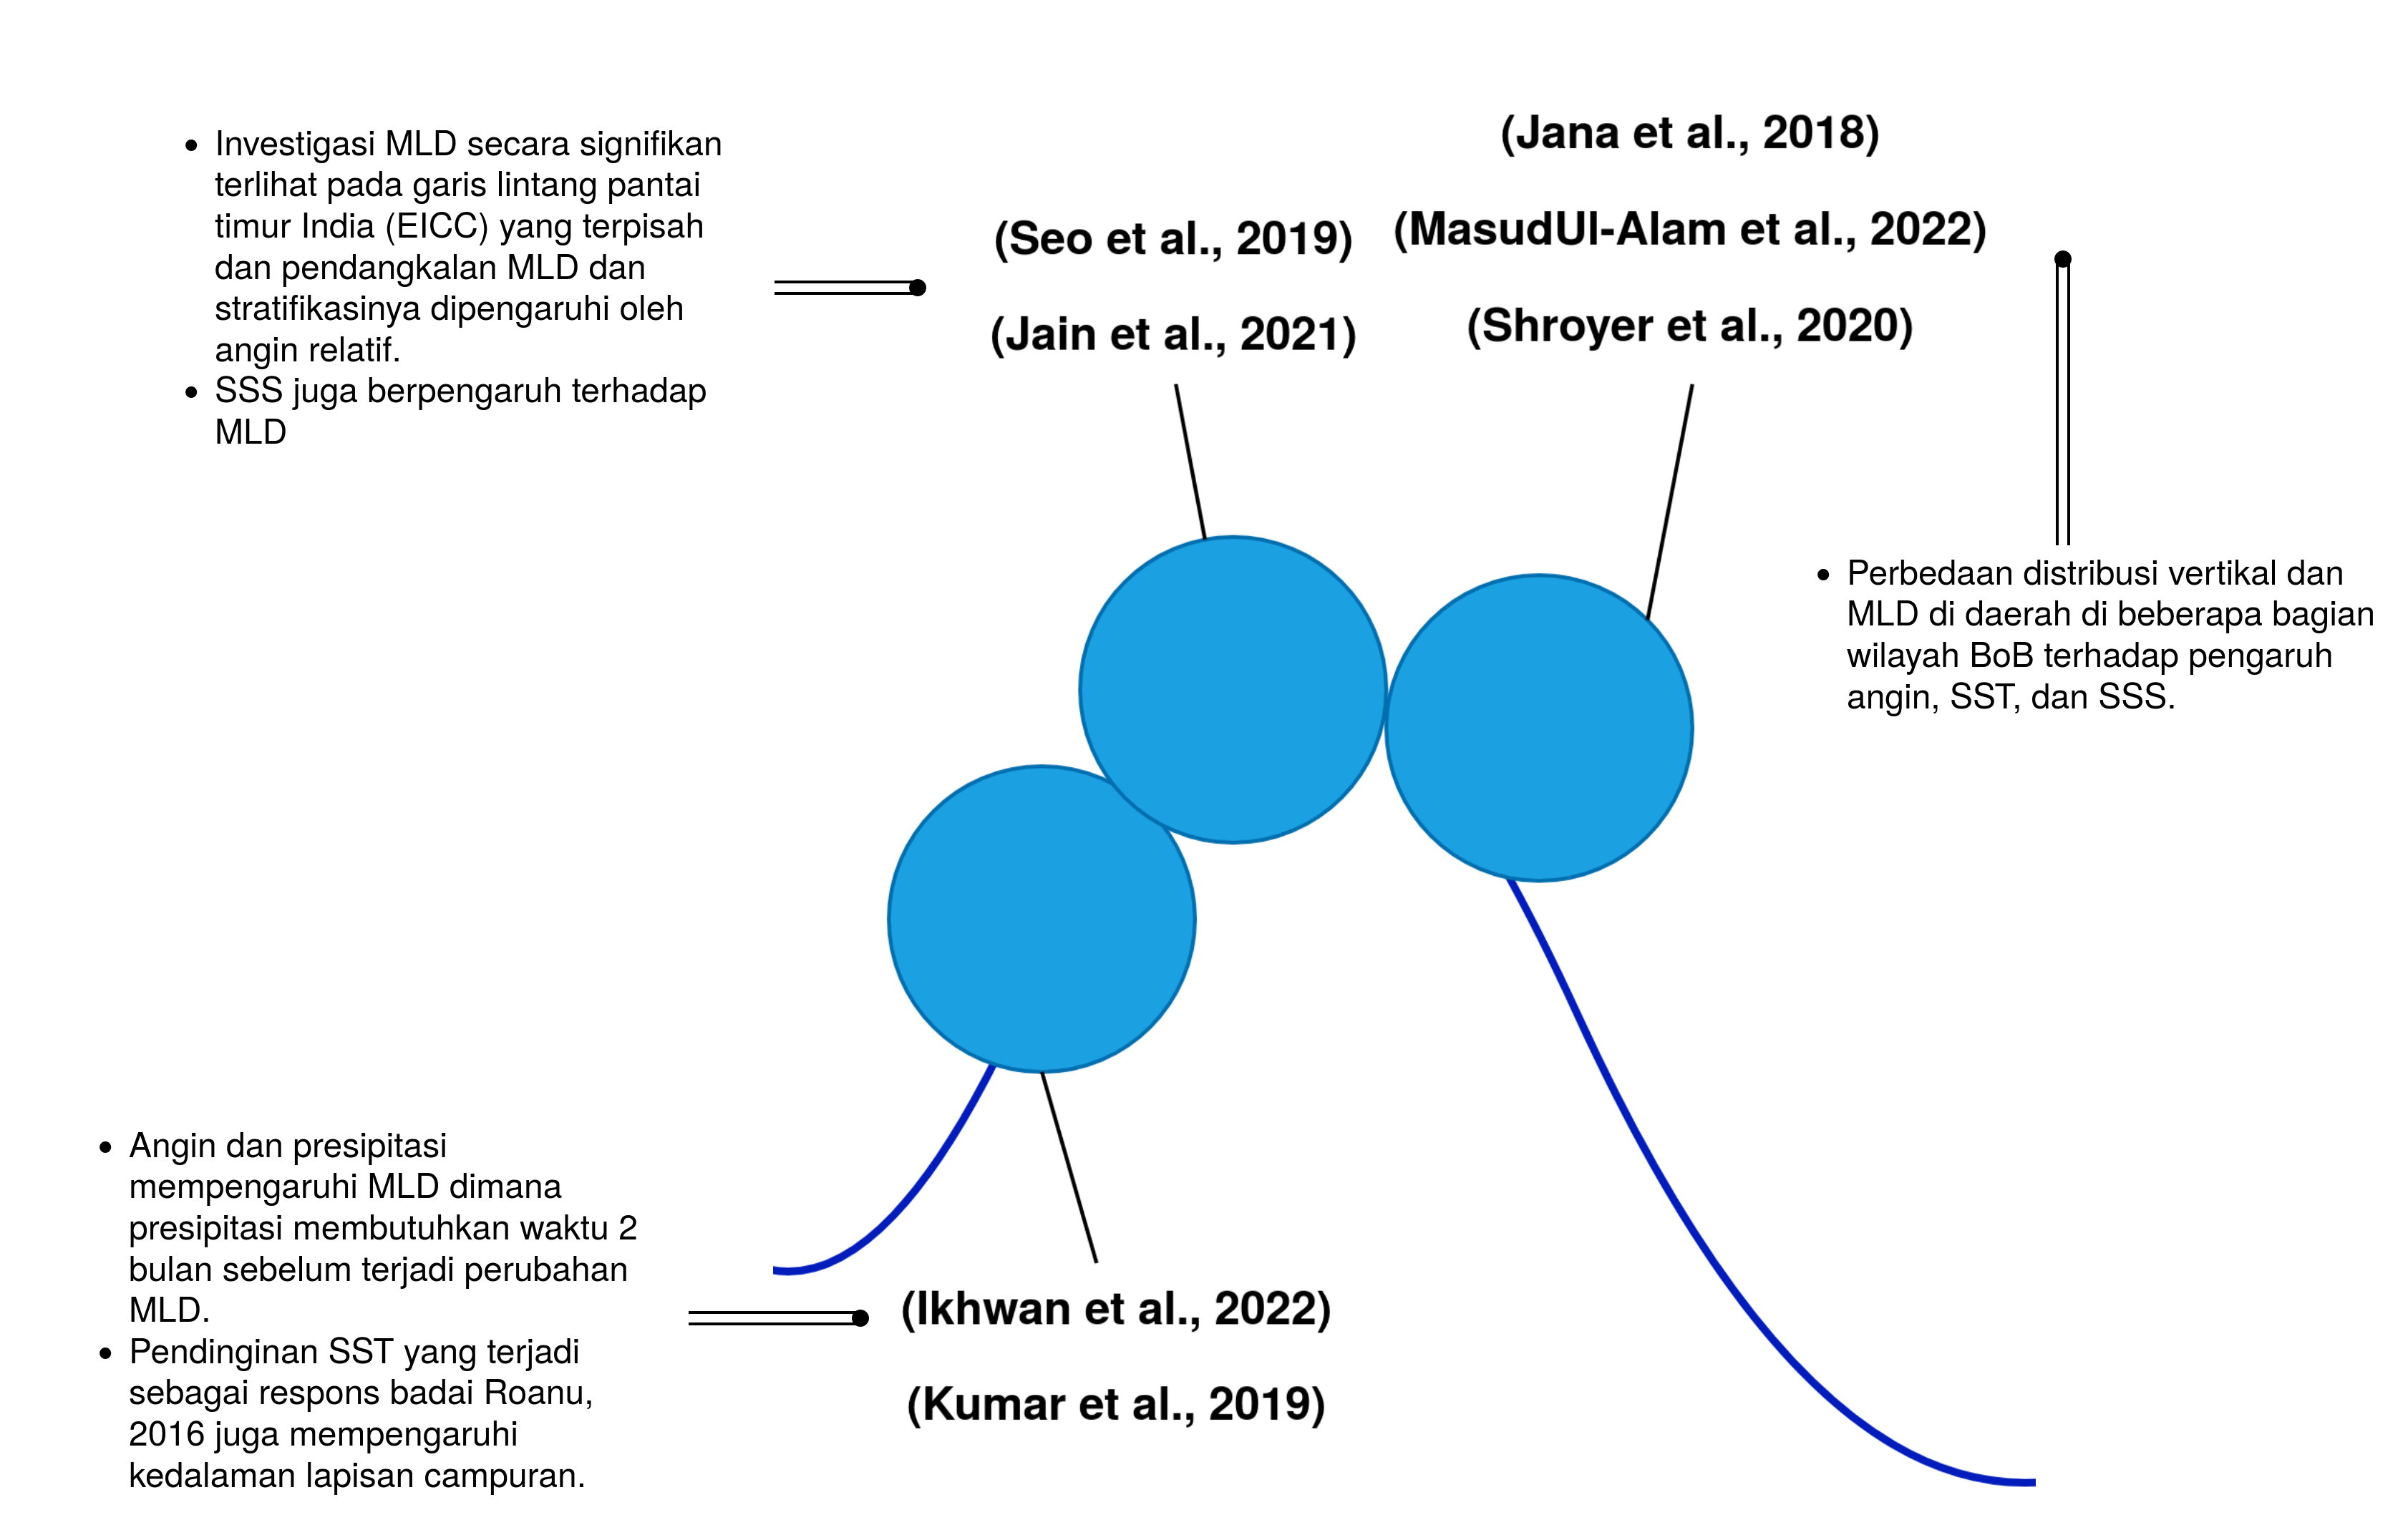
\includegraphics[width=10cm]{intro-2_1}
	\end{figure}
%	\newpage
	\begin{figure}[H]
		\centering
		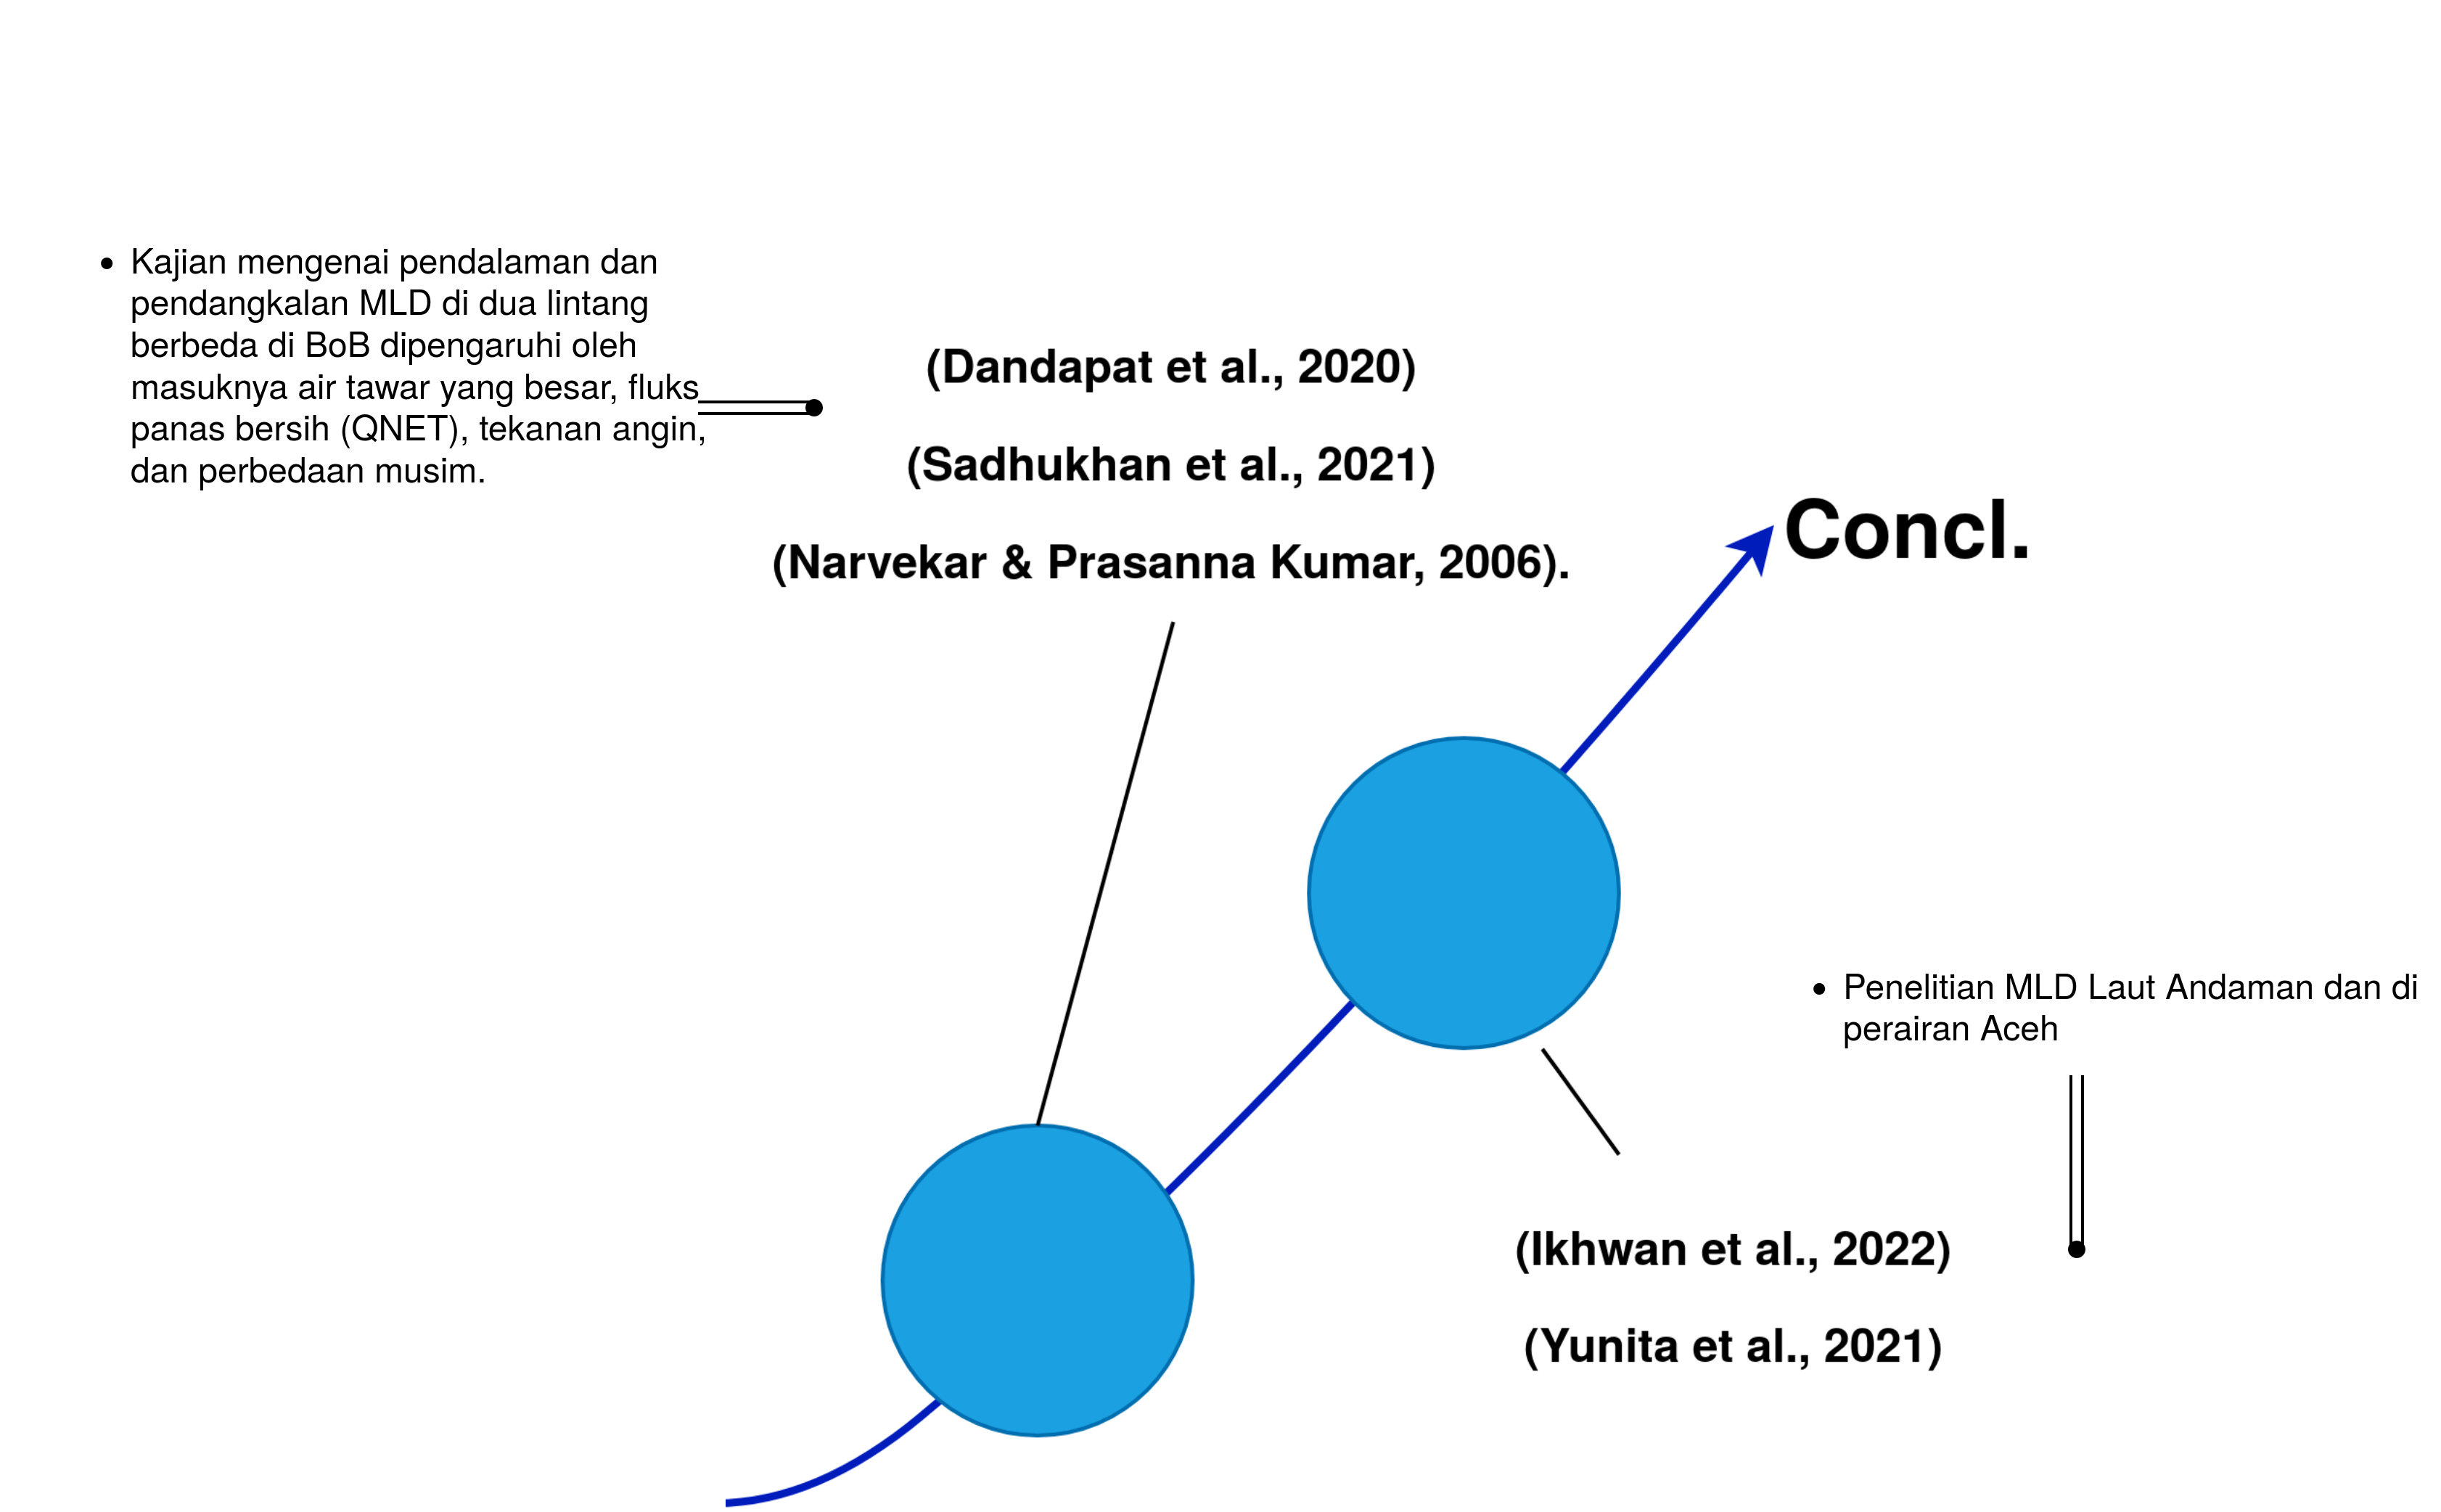
\includegraphics[width=10cm]{intro-3_1}
	\end{figure}
\end{frame}

\subsection{Rumusan Masalah}
\begin{frame}
	\frametitle{Rumusan Masalah}
	\textbf{Masalah utama},
	\colorbox{lightgray}{Bagaimana pengaruh parameter meteorologi}\\  \colorbox{lightgray}{terhadap kedalaman lapisan campuran (\textit{Mixed Layer Depth})} \\
	\colorbox{lightgray}{di Perairan Aceh?} 
	
	\textbf{Subpertanyaan},
	\begin{itemize}
		\item {\small Bagaimana analisis kedalaman lapisan campuran (MLD) di wilayah perairan Aceh dalam 12 bulan pada tahun 2021?} 
		\item {\small Bagaimana analisis model iklim untuk parameter-parameter meteorologi \textit{2m air temperature, 2m specific humidity, convective precipitation rate, sea level pressure, wind stress U}, dan \textit{wind stress V} selama 22 tahun, tahun 2000 - 2021?}
		\item {\small Bagaimana hubungan parameter meteorologi terhadap analisis kedalaman lapisan campuran (MLD) di wilayah perairan Aceh?}
	\end{itemize}
\end{frame}

\subsection{Tujuan Penelitian}
\begin{frame}
\frametitle{Tujuan Penelitian}
	Mencari tahu pengaruh parameter meteorologi terhadap kedalaman lapisan campuran (\textit{Mixed Layer Depth}) di Perairan Aceh dengan cara

	\begin{itemize}
		\item {\small Analisis kedalaman lapisan campuran (MLD) di wilayah perairan Aceh dalam 12 bulan pada tahun 2021} 
		\item {\small Analisis model iklim untuk parameter-parameter meteorologi \textit{2m air temperature, 2m specific humidity, convective precipitation rate, sea level pressure, wind stress U}, dan \textit{wind stress V} selama 22 tahun, tahun 2000 - 2021}
		\item {\small Hubungan parameter meteorologi terhadap analisis kedalaman lapisan campuran (MLD) di wilayah perairan Aceh}
	\end{itemize}
\end{frame}

\subsection{Urgensi dan Kebaruan Penelitian}
\begin{frame}
	\frametitle{Urgensi dan Kebaruan Penelitian}
	Sejauh pengamatan kami, studi secara detail terkait 6 parameter meteorologi dan dampaknya terhadap lapisan vertikal di wilayah perairan Aceh belum pernah dilakukan sebelumnya. Oleh karena itu, dirasa penting untuk melakukan penelitian ini guna mengetahui pengaruh paramater meteorologi terhadap kedalaman lapisan campuran (MLD).
\end{frame}

\subsection{Manfaat Penelitian}
\begin{frame}
	\frametitle{Manfaat Penelitian}
	\begin{itemize}
		\item Memberikan kontribusi ilmiah dan memperkaya pengetahuan tentang kedalaman lapisan campuran atau MLD.
		\item Dari periodesitas model iklim yang diperoleh akan bermanfaat untuk tujuan fishing ground, mitigasi perubahan iklim dan bencana hidro-oseanografi, tata ruang dan konservasi laut, dan sumber energi terbarukan.
	\end{itemize}
\end{frame}

\section{Tinjauan Pustaka}
\begin{frame}
	\centering
	\begin{figure}[H]
		\centering
		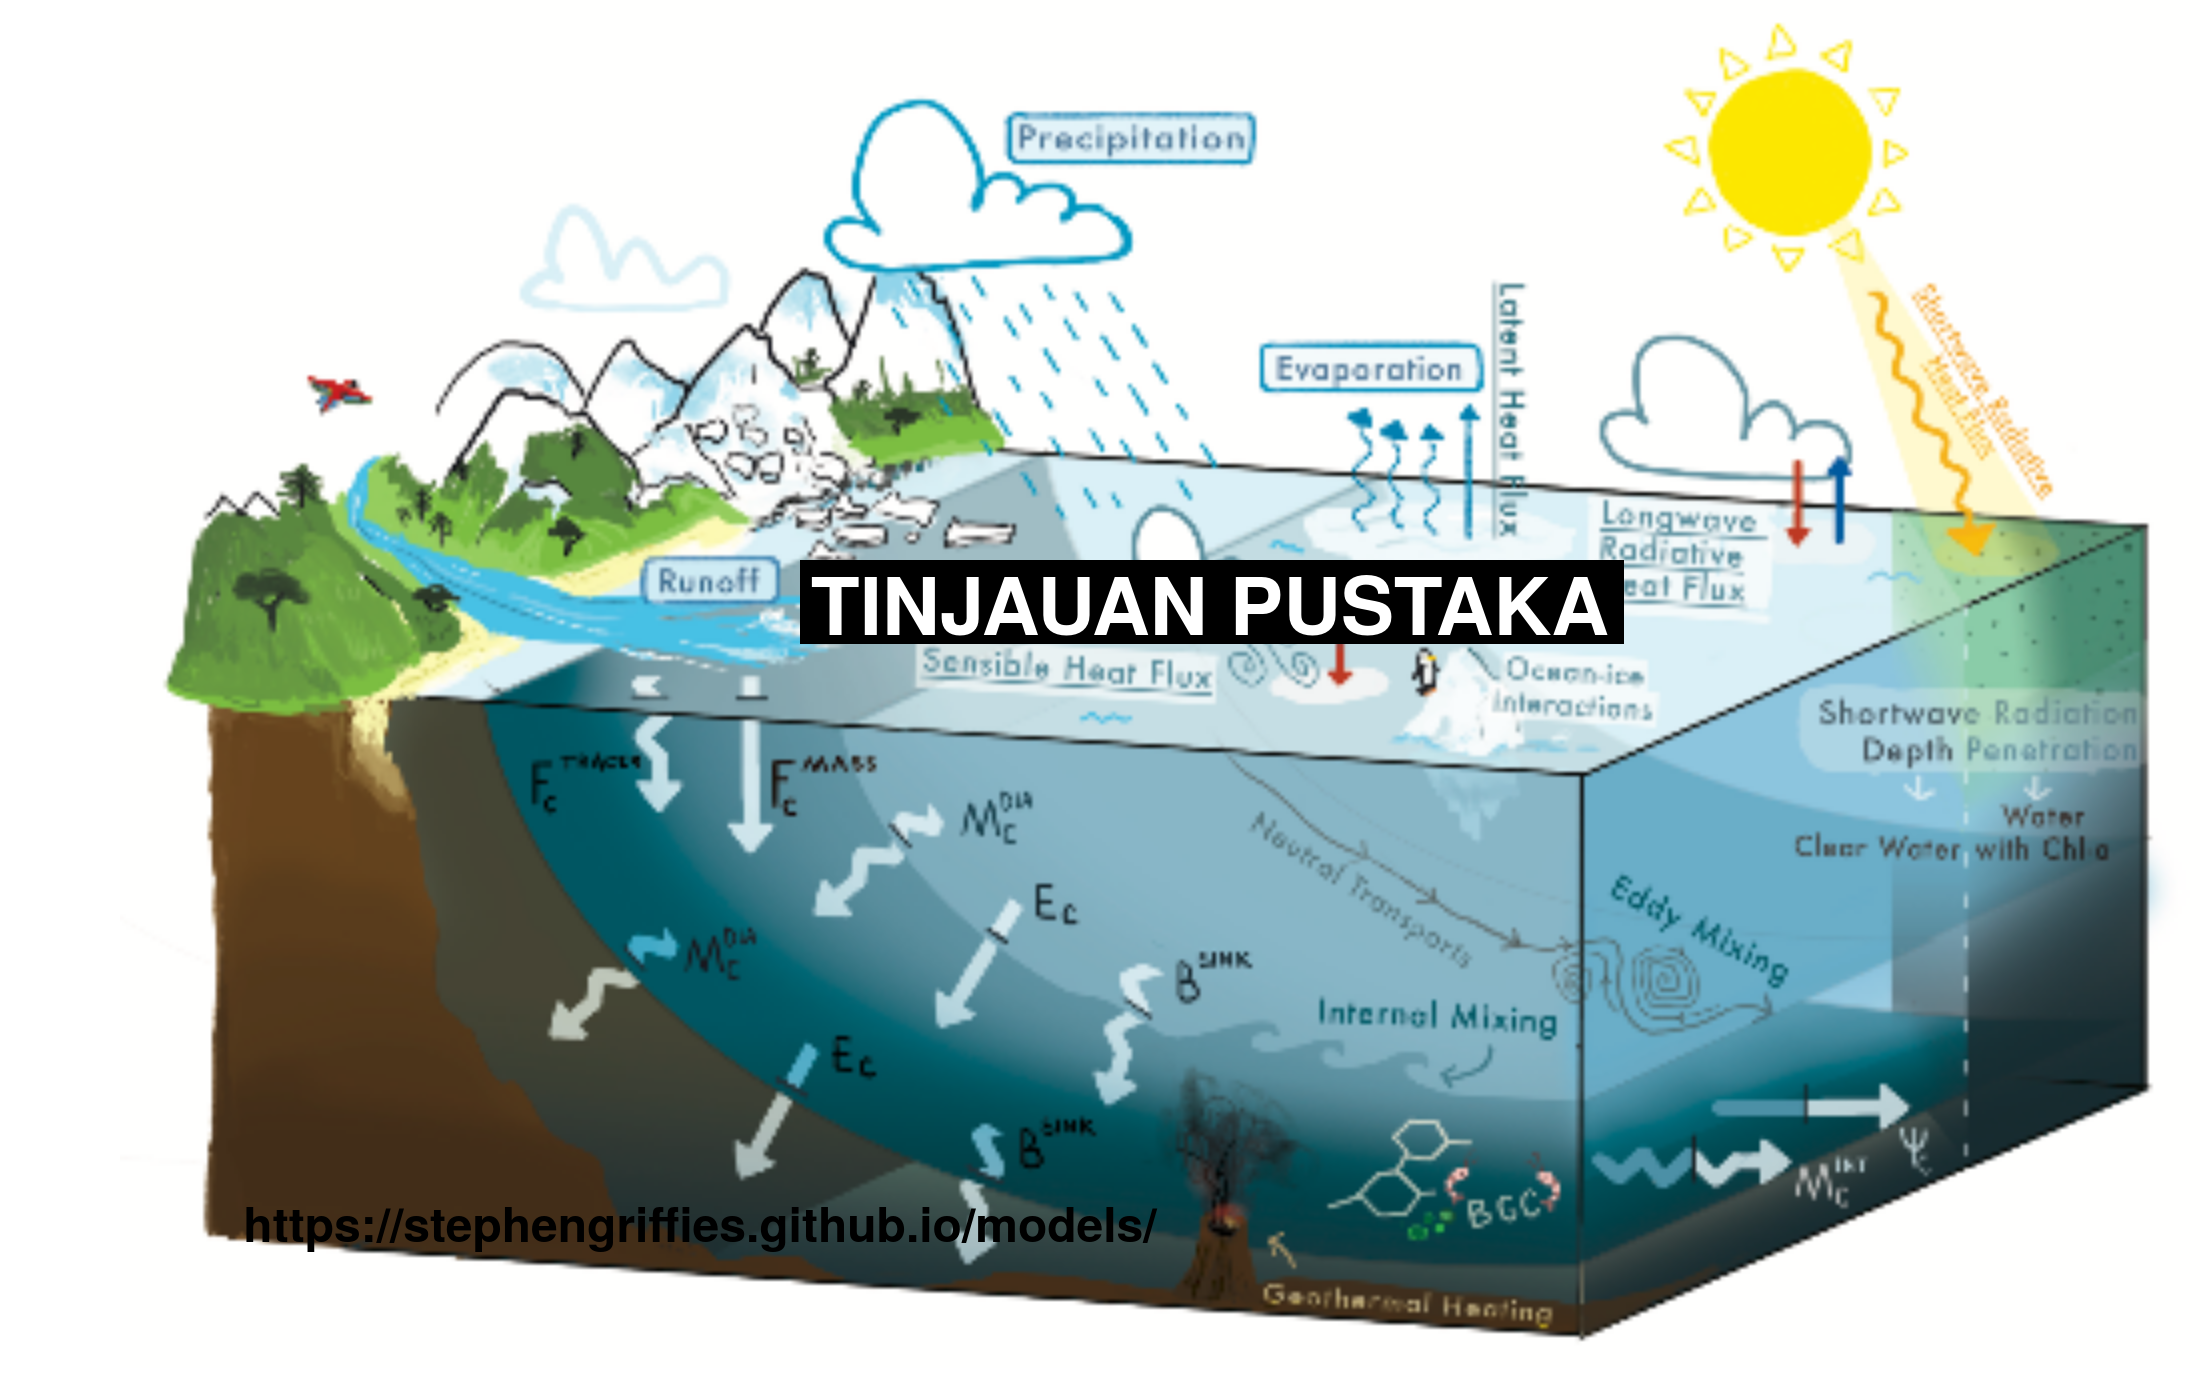
\includegraphics[width=10cm]{Bg_2}
	\end{figure}
\end{frame}
\subsection{Persamaan Gerak Fluida}
\begin{frame}
	\frametitle{Persamaan Gerak Fluida}
	\begin{figure}[H]
		\centering
		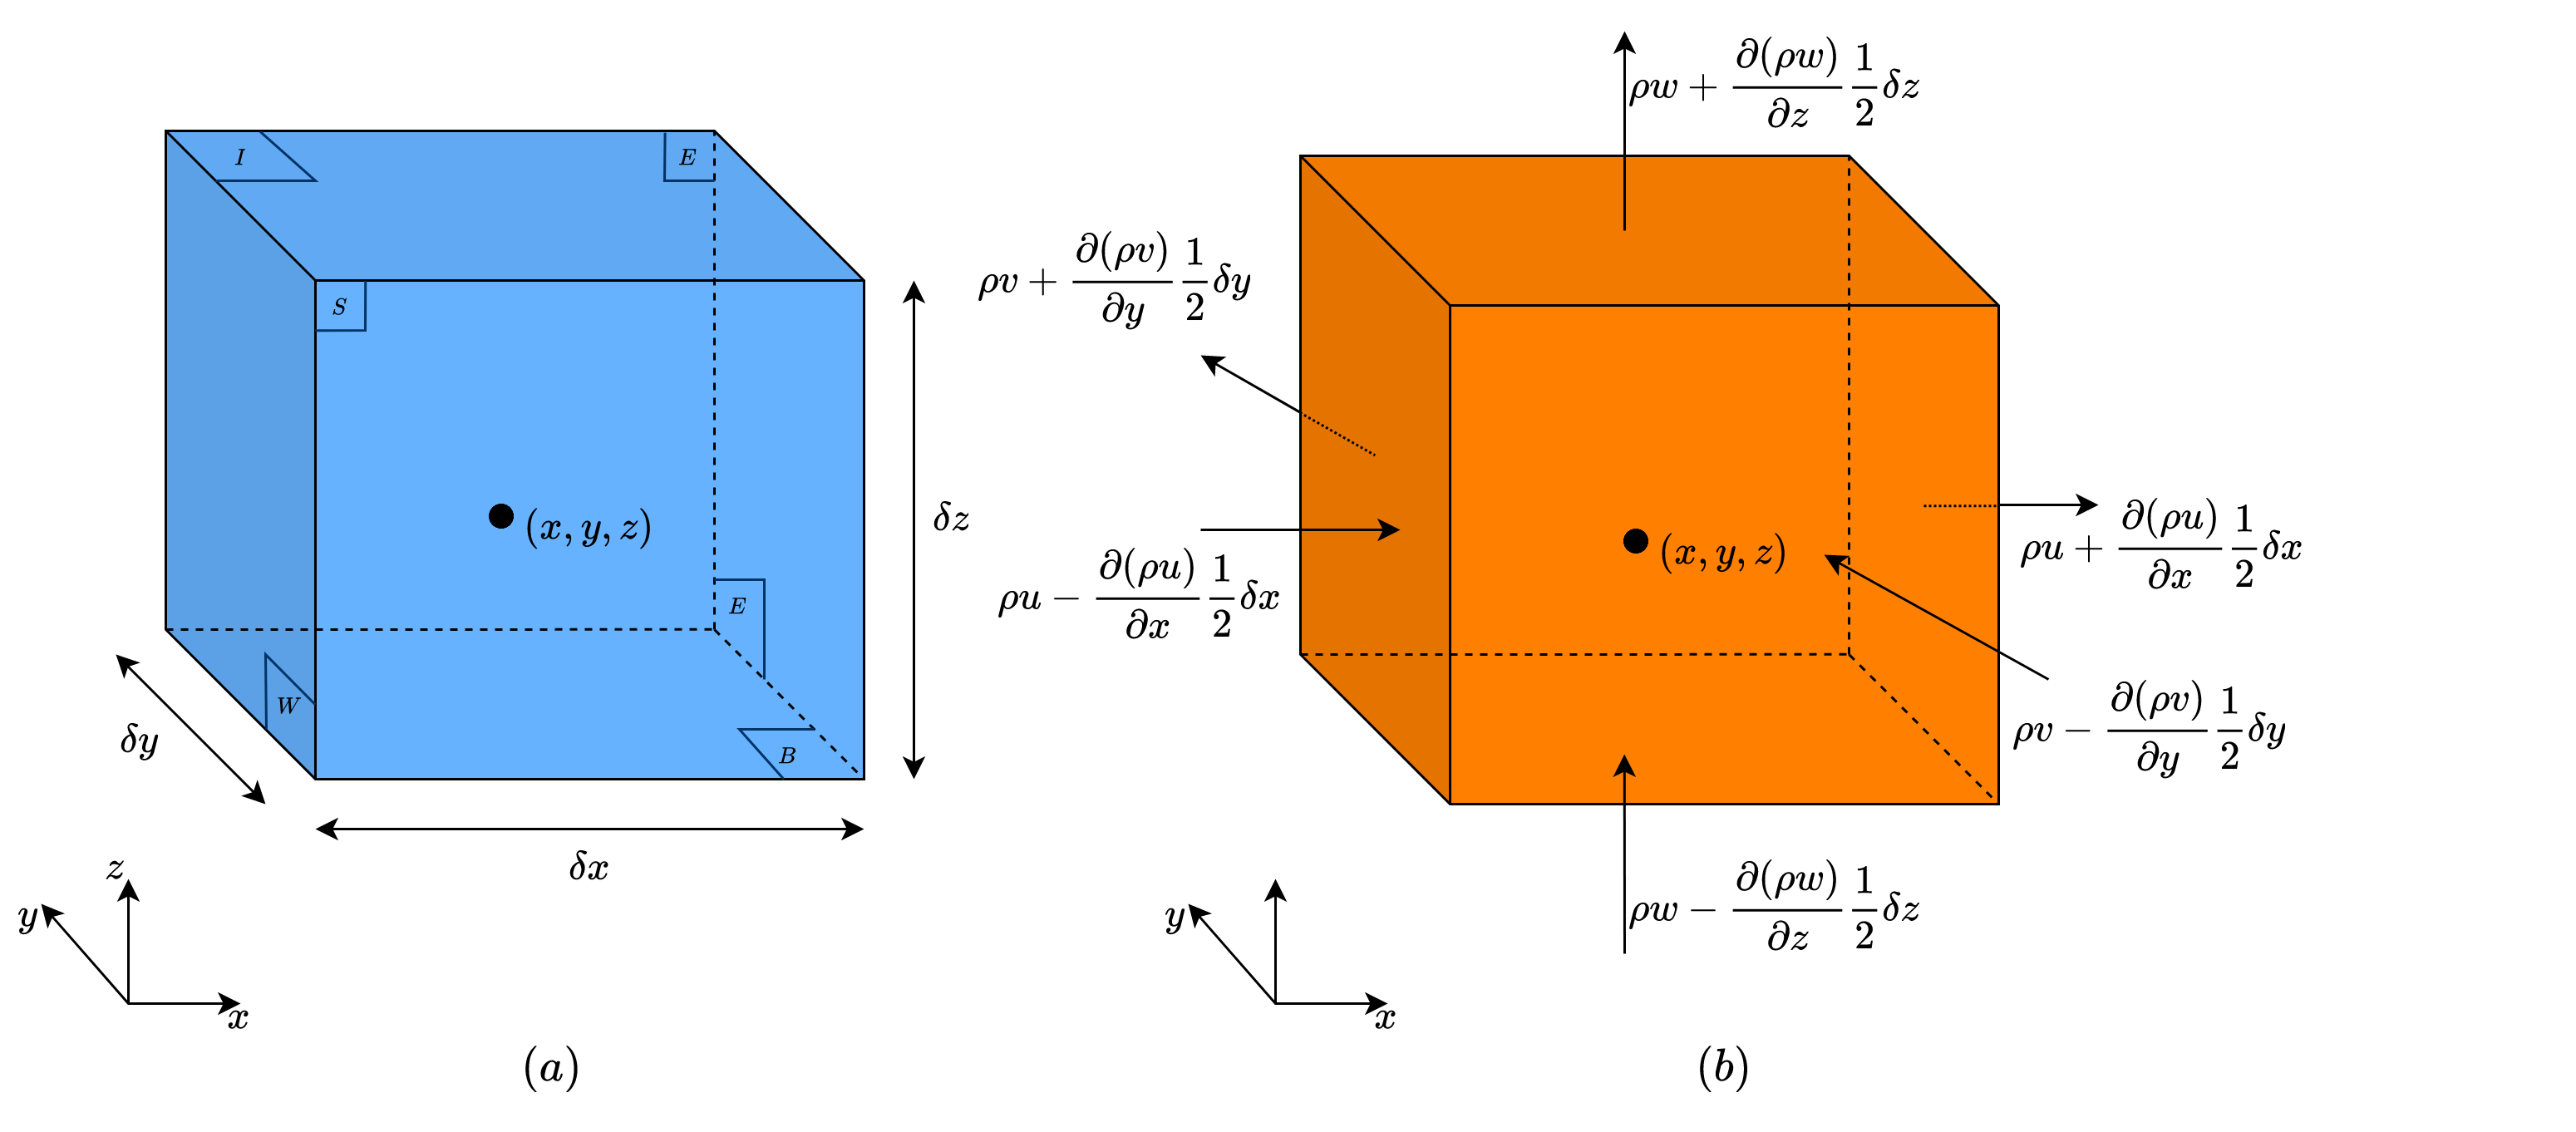
\includegraphics[width=10cm]{cube.png}
		\captionsetup{labelformat=empty}
		\caption{Gambar 2.1. (a) Ilustrasi partikel sebagai sifat fisis fluida. (b) Aliran massa jenis masuk dan keluar. Gambar direproduksi dari (Versteeg \& Malalasekera, 2007)}
		\label{fig:cube}
	\end{figure}
\end{frame}

\subsection{Persamaan Primitif}
\begin{frame}[allowframebreaks]
	\frametitle{Persamaan Primitif}
	$\;$ \\
	$\;$ \\
	$\;$ \\
	Model OGCM $\rightarrow$ persamaan Navier-Stokes, menggunakan hipotesis (Gurvan et al., 2022),
	\begin{itemize}
		\item {\small Hipotesis Boussinesq $\rightarrow \rho = \rho(T,S,p)$}
		\item {\small Hipotesis hidrostatik $\rightarrow \frac{\partial p}{\partial z} = -\rho g$}
		\item {\small Hipotesis tak termampatkan $\rightarrow \nabla \;.\; U = 0$}.
	\end{itemize}
	\newpage
		- Persamaan kesetimbangan momentum
	\begin{equation}
		\begin{aligned}
			\frac{\partial U_h}{\partial t} = - \left[(\nabla \times U) \times U + \frac{1}{2}\nabla (U^2)\right]_h - f \; k \times U_h \\
			- \frac{1}{\rho_o}\nabla_h p + D^U + F^U.
		\end{aligned}
	\end{equation}

	- Persamaan konservasi panas dan salinitas
	\begin{equation}
		\begin{aligned}
			\frac{\partial T}{\partial t} &= - \nabla \; . \; (T\;U)  + D^U + F^U \\
			\frac{\partial S}{\partial t} &= - \nabla \; . \; (S\;U)  + D^U + F^U
		\end{aligned}
	\end{equation}
\end{frame}

\subsection{Arakawa C-grid}
\begin{frame}[allowframebreaks]
	\frametitle{Arakawa C-grid}	

	\begin{figure}[H]
	\centering
	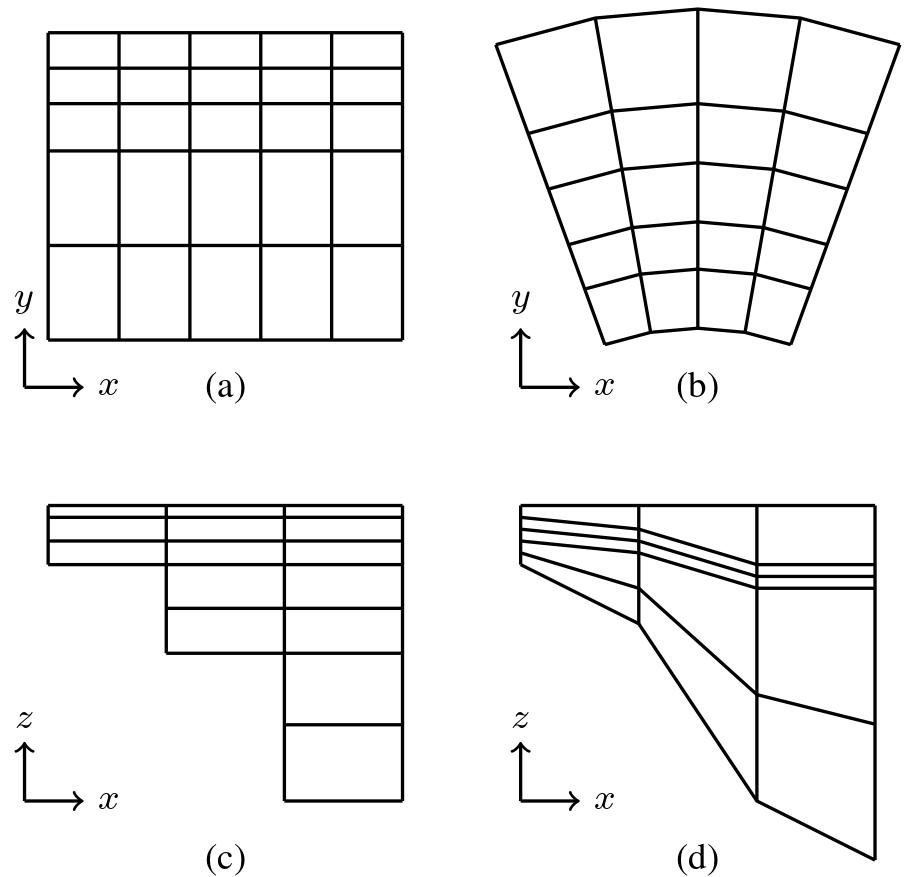
\includegraphics[width=4cm]{grid.jpg}
	\captionsetup{labelformat=empty}
	\caption{Gambar 2.2. Jenis grid dalam pemodelan laut. Di bidang horizontal: (a) grid persegi, (b) grid lengkung, di bidang vertikal: (c) grid level z, (d) grid level s (Delandmeter \& van Sebille, 2019)}
	\label{fig:grid}
	\end{figure}
	$\;$ \\
	\begin{figure}[H]
		\centering
		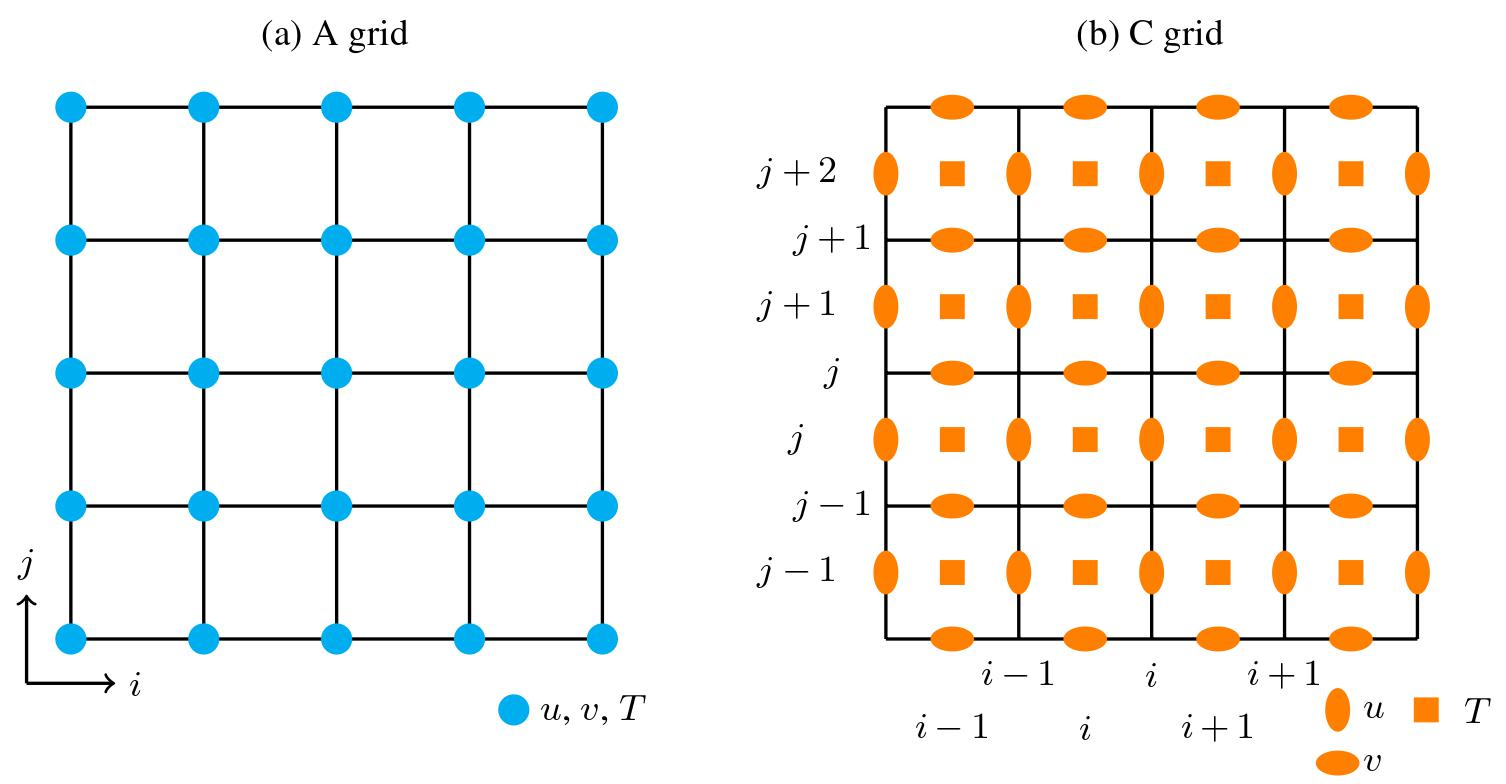
\includegraphics[width=6cm]{arakawa.jpg}
		\captionsetup{labelformat=empty}
		\caption{Gambar 2.3. Grid Arakawa: (a) Grid A dan (b) Grid C (Delandmeter \& van Sebille, 2019)}
			\label{fig:arakawa}
%			\medspace
			\tiny
		Grid A adalah satu-satunya \textit{unstaggered grid} dalam grid Arakawa dimana variabel-variabelnya (\textit{zonal velocity (u), meridional velocity (v), tracers (T)}) hanya terdapat pada titik sudut grid, berbeda dengan grid C yang berada di sisi dan tengah grid. $i$ dan $j$ adalah indeks yang merepresentasikan variabel kolom dan baris dimana variabel disimpan.
	\end{figure}	
\end{frame}

\subsection{Model Iklim}
\begin{frame}[allowframebreaks]
	\frametitle{Model Iklim}
	Persamaan untuk siklus musiman (Crawley, 2012, p. 793) secara lengkap diberikan oleh,
	\begin{equation}\label{eq:sm}
		y = \alpha + \beta \sin(2\pi t)+\gamma \cos(2\pi t) + \epsilon
	\end{equation}
	dengan $\alpha$ adalah konstanta pergesaran vertikal, $\beta$ adalah amplitude dari gelombang sinus, $\gamma$ adalah amplitude dari gelombang kosinus, $t$ adalah waktu, dan $\epsilon$ adalah elemen residual yang mungkin mewakili komponen white-noise tidak beraturan dalam proses yang mendasari data.	
\end{frame}

\subsection{Kedalaman Lapisan Campuran}
\begin{frame}[allowframebreaks]
	\frametitle{Kedalaman Lapisan Campuran}
		\begin{figure}[H]
			\centering
			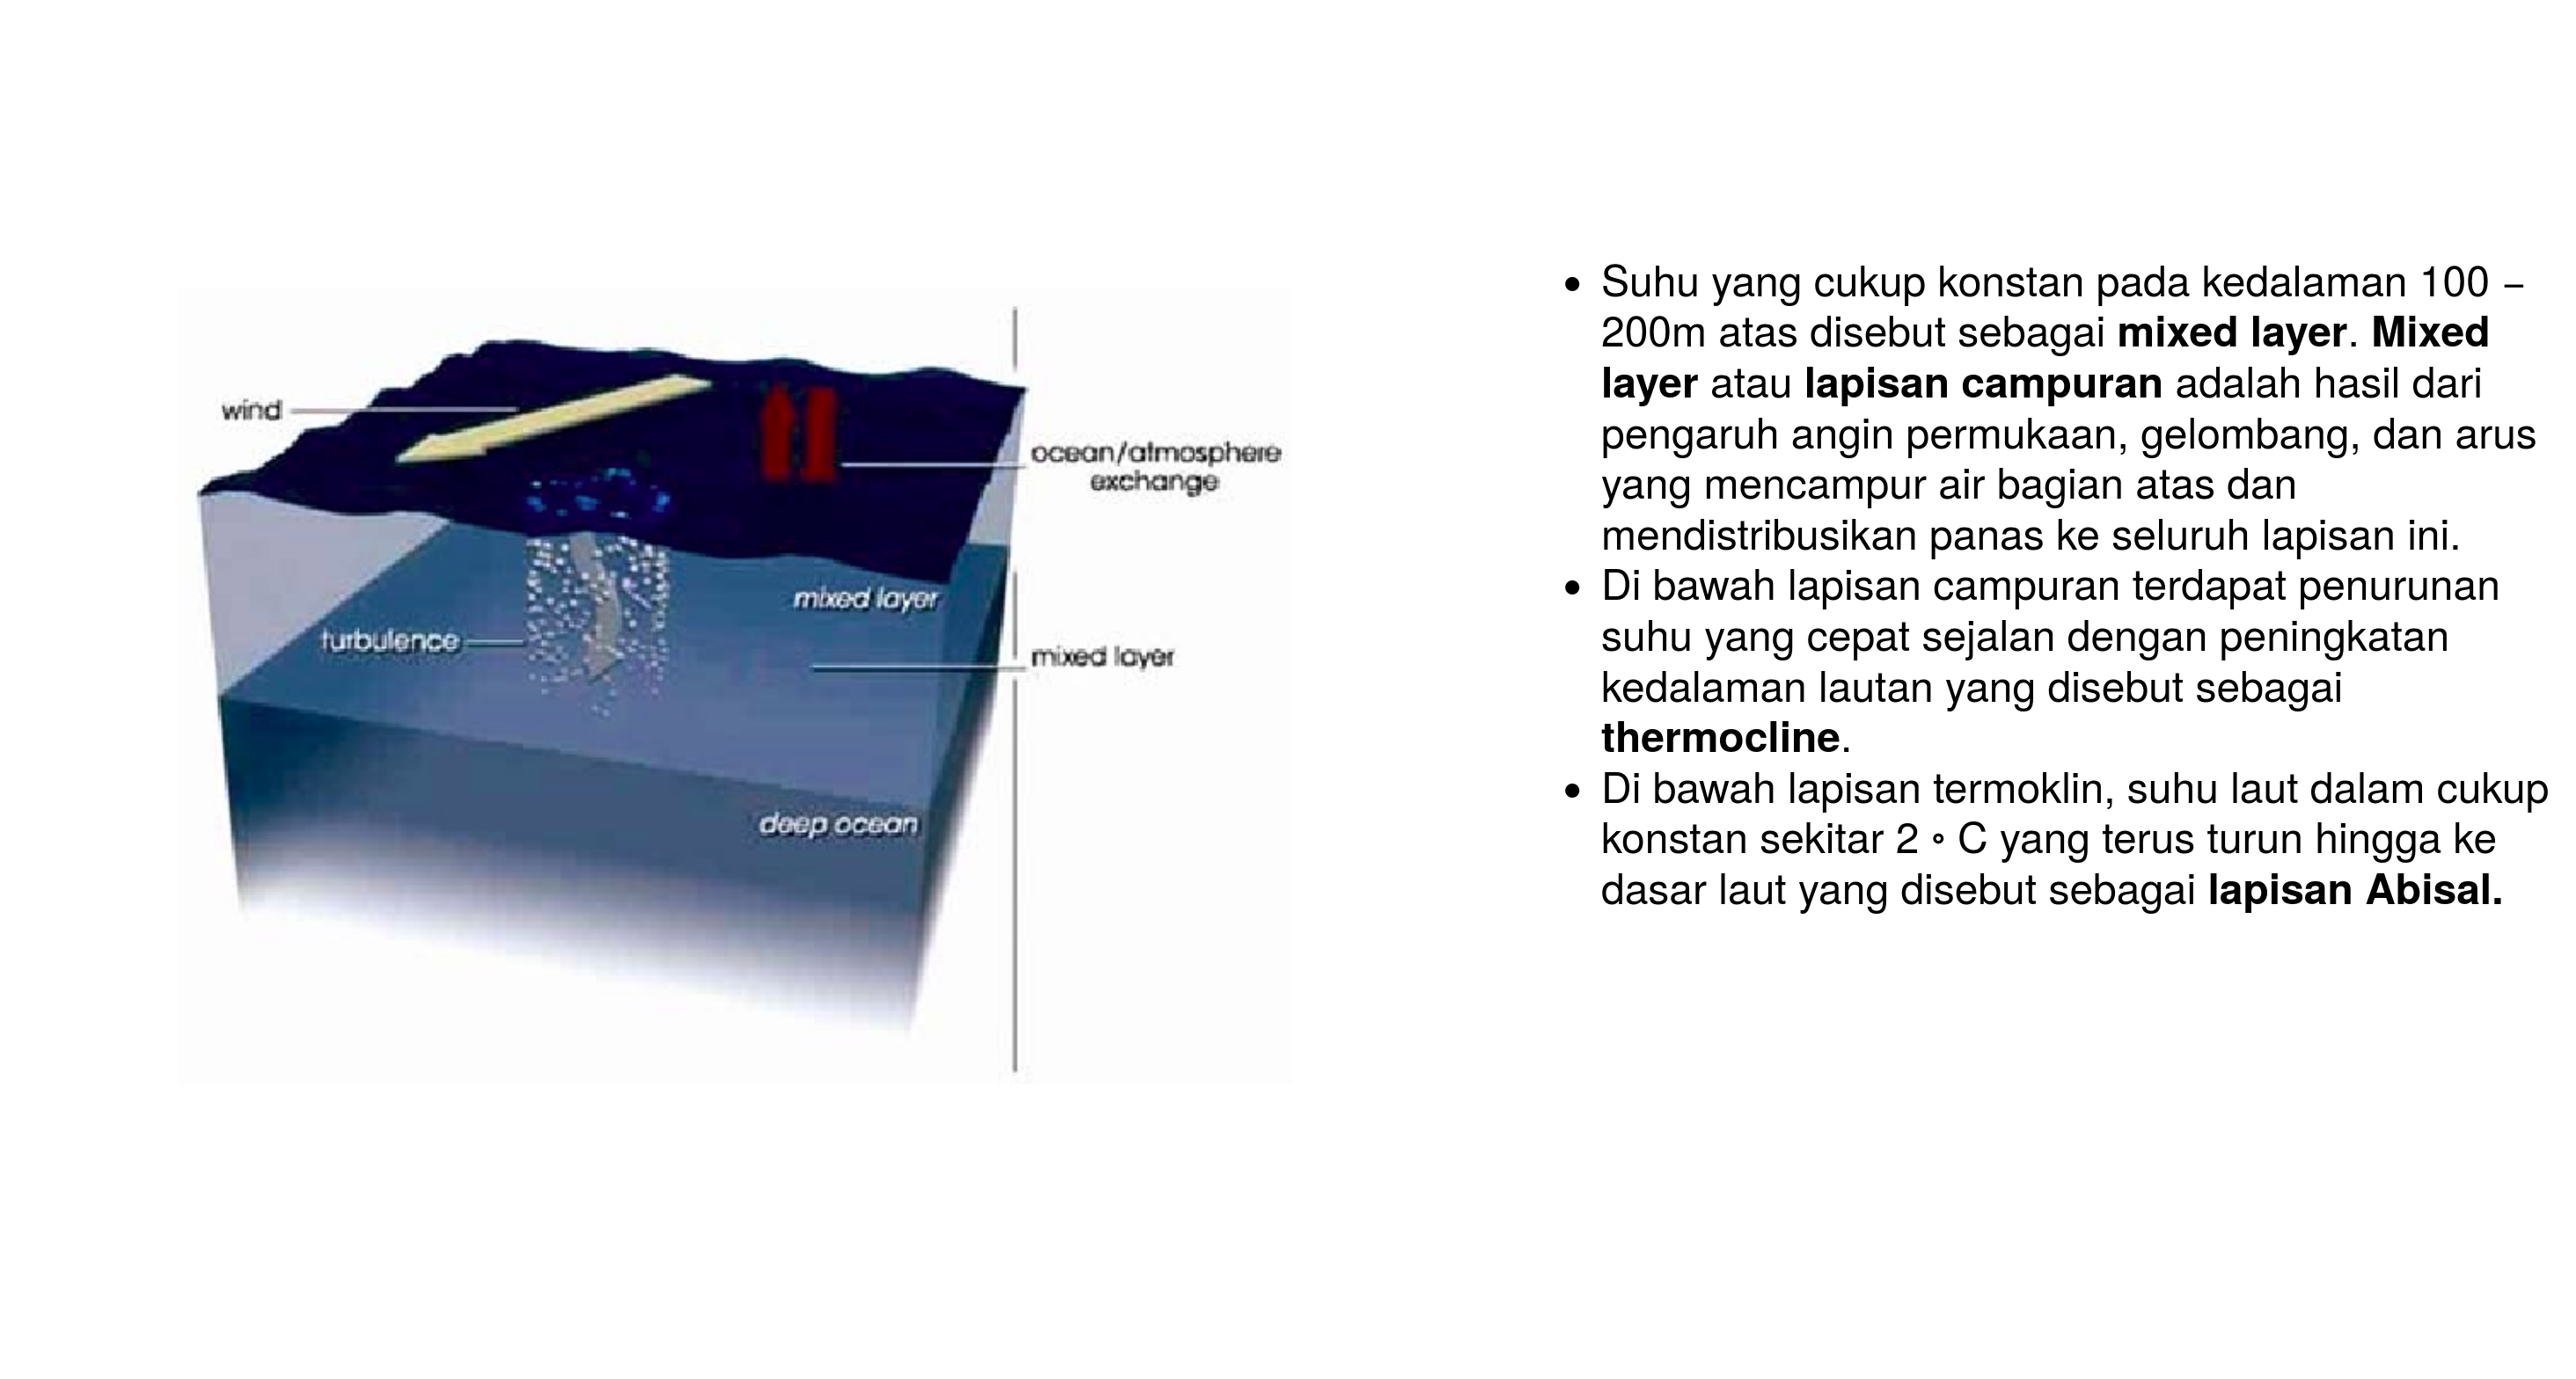
\includegraphics[width=10cm]{mld_1.png}
		\end{figure}	
		\begin{figure}[H]
		\centering
		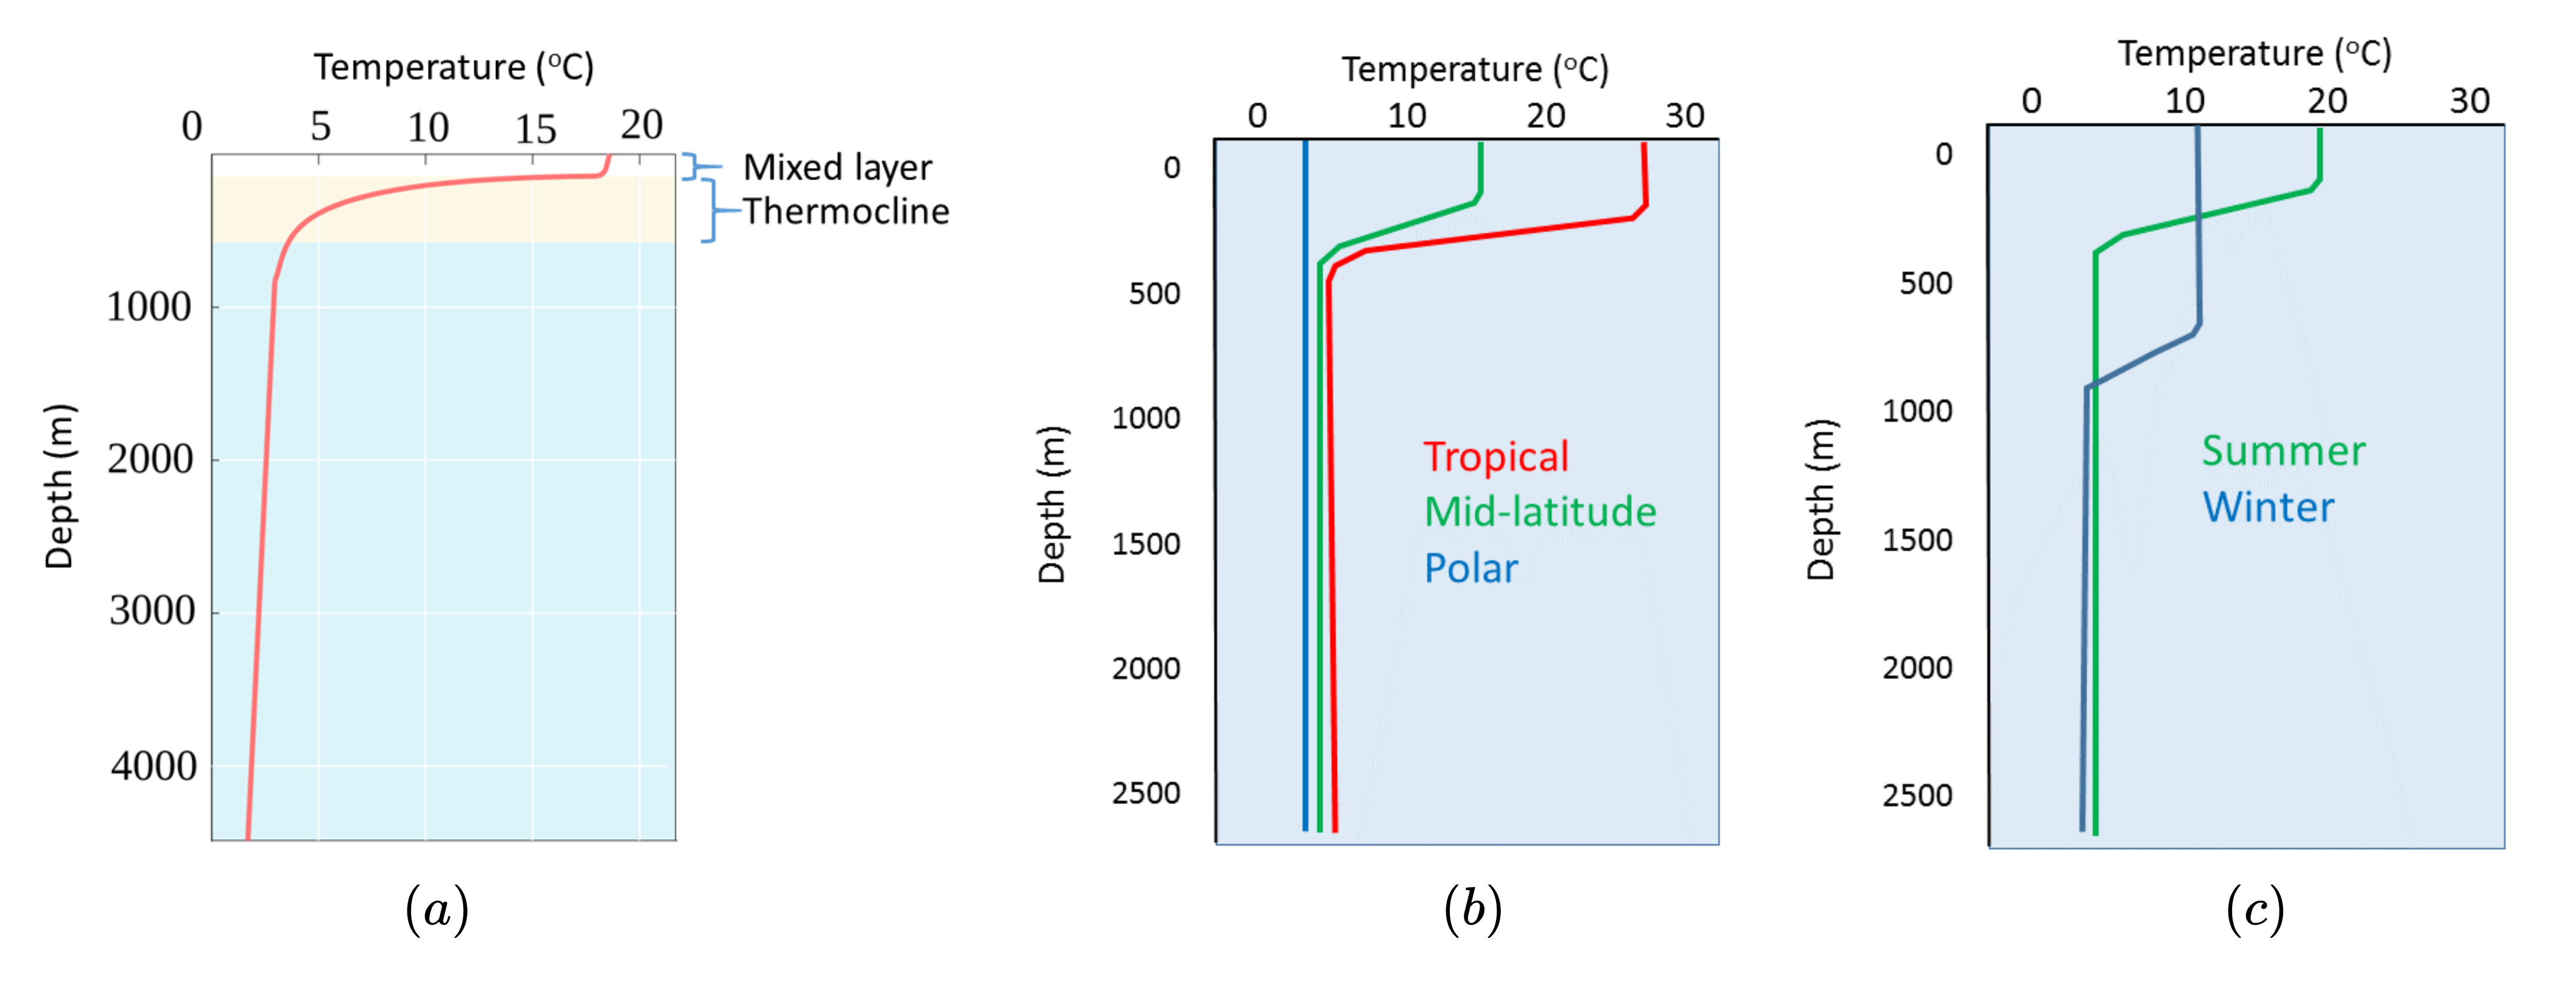
\includegraphics[width=9cm]{mld_theory.png}
		\captionsetup{labelformat=empty}
		\caption{Gambar 2.4. Ilustrasi kedalaman lapisan campuran}
		\tiny
		(a) Profil suhu laut terbuka yang khas untuk wilayah lintang tengah, menunjukkan lapisan campuran, termoklin yang curam, dan suhu yang relatif stabil di kedalaman, (b) Profil suhu representatif untuk daerah tropis, lintang tengah, dan kutub, dan (c) Di daerah beriklim sedang, lapisan campuran lebih dalam dan termoklin kurang menonjol di musim dingin dibandingkan dengan musim panas (Webb, 2021)
		\label{fig:mld_theory}
	\end{figure}	
\end{frame}

\section{Metodologi Penelitian}
\begin{frame}
	\centering
	\begin{figure}[H]
		\centering
		
\includegraphics[width=10cm]{Bg_3}
	\end{figure}
\end{frame}
\subsection{Domain Penelitian}
\begin{frame}[allowframebreaks]
	\frametitle{Domain Penelitian}
	\begin{figure}[H]
		\centering
		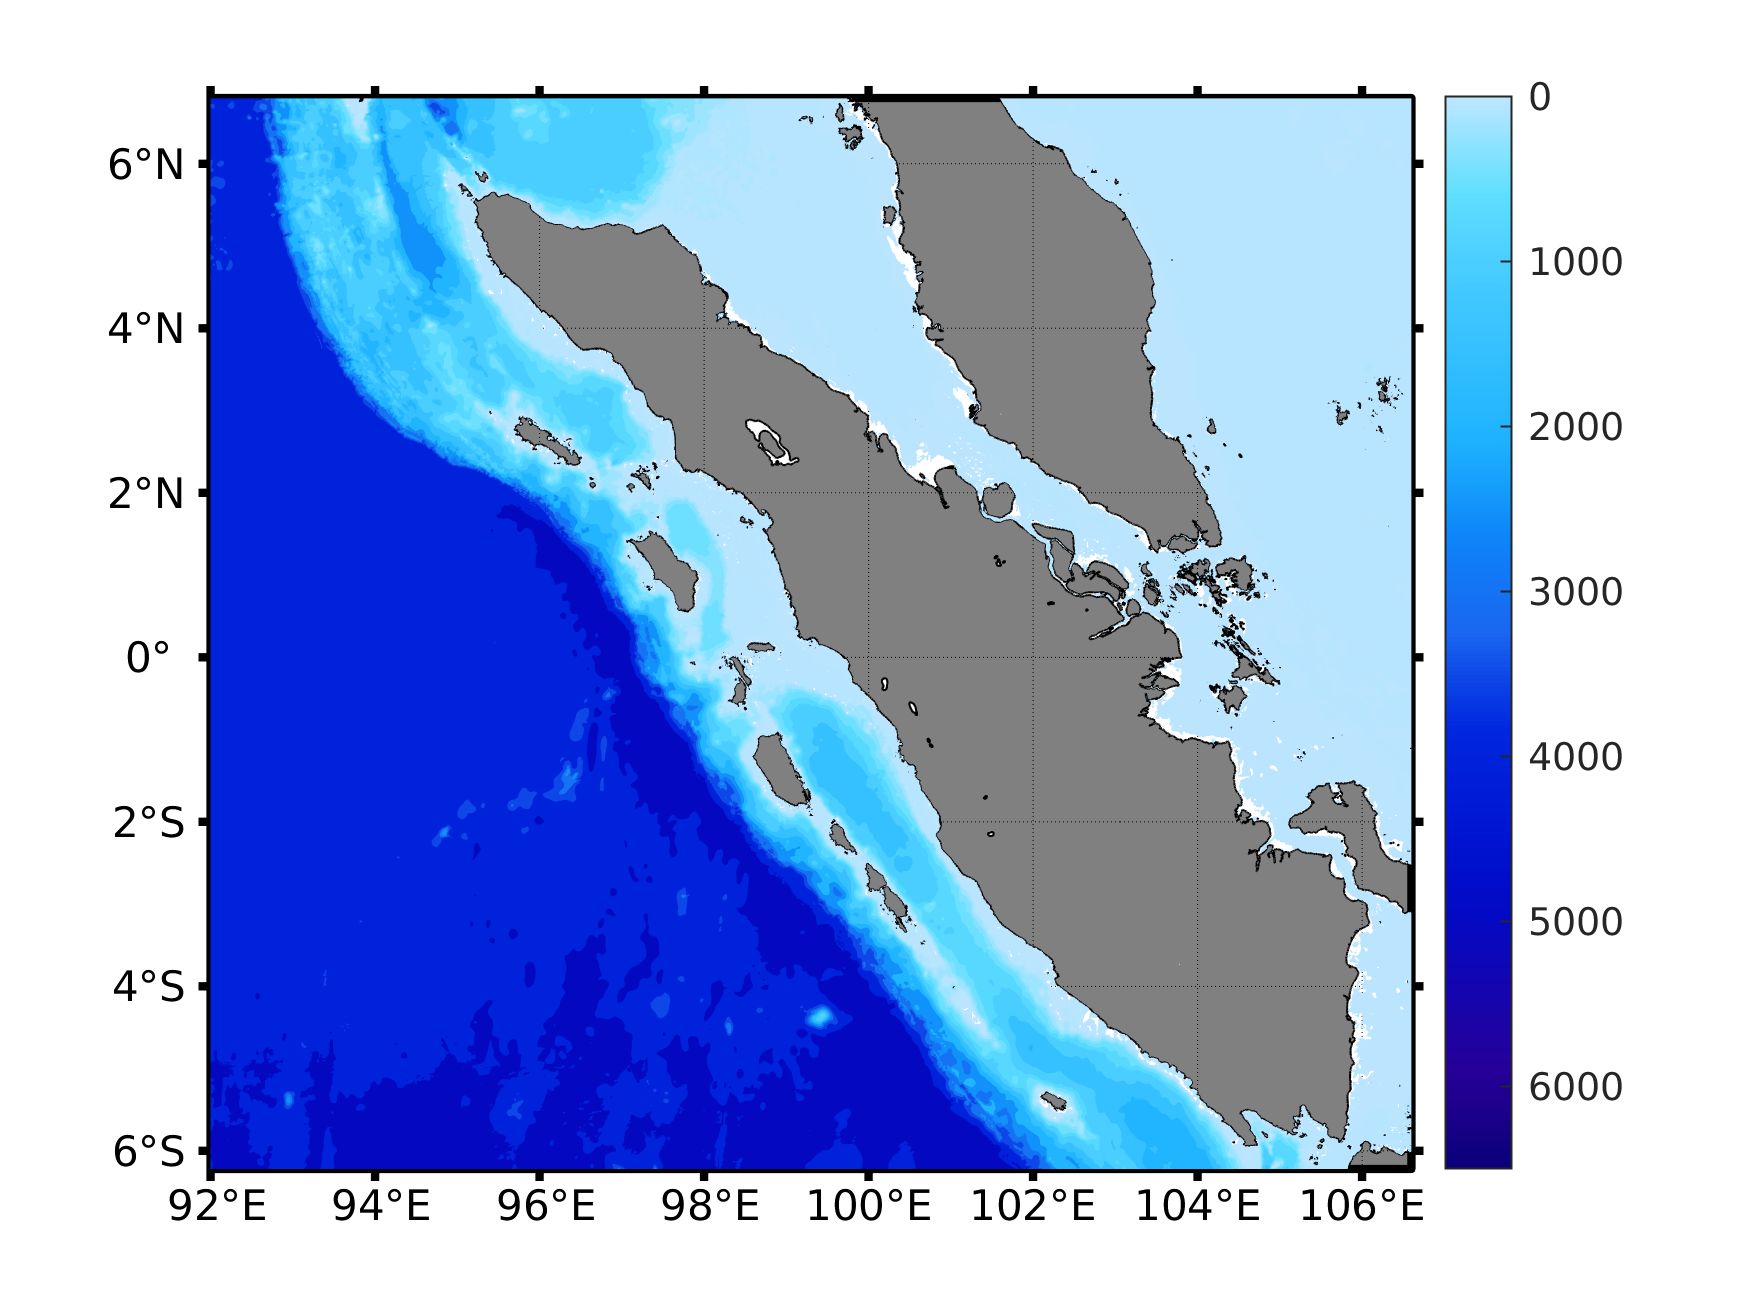
\includegraphics[width=7cm]{Topo_1}
		\captionsetup{labelformat=empty}
		\caption{Gambar 3.1. Data batimetri domain perairan Aceh, Selat Malaka, Bagian Laut Cina Selatan, dicuplik dari SRTM15+}
		\label{fig:domain}
	\end{figure}
	\begin{figure}[H]
		\centering
		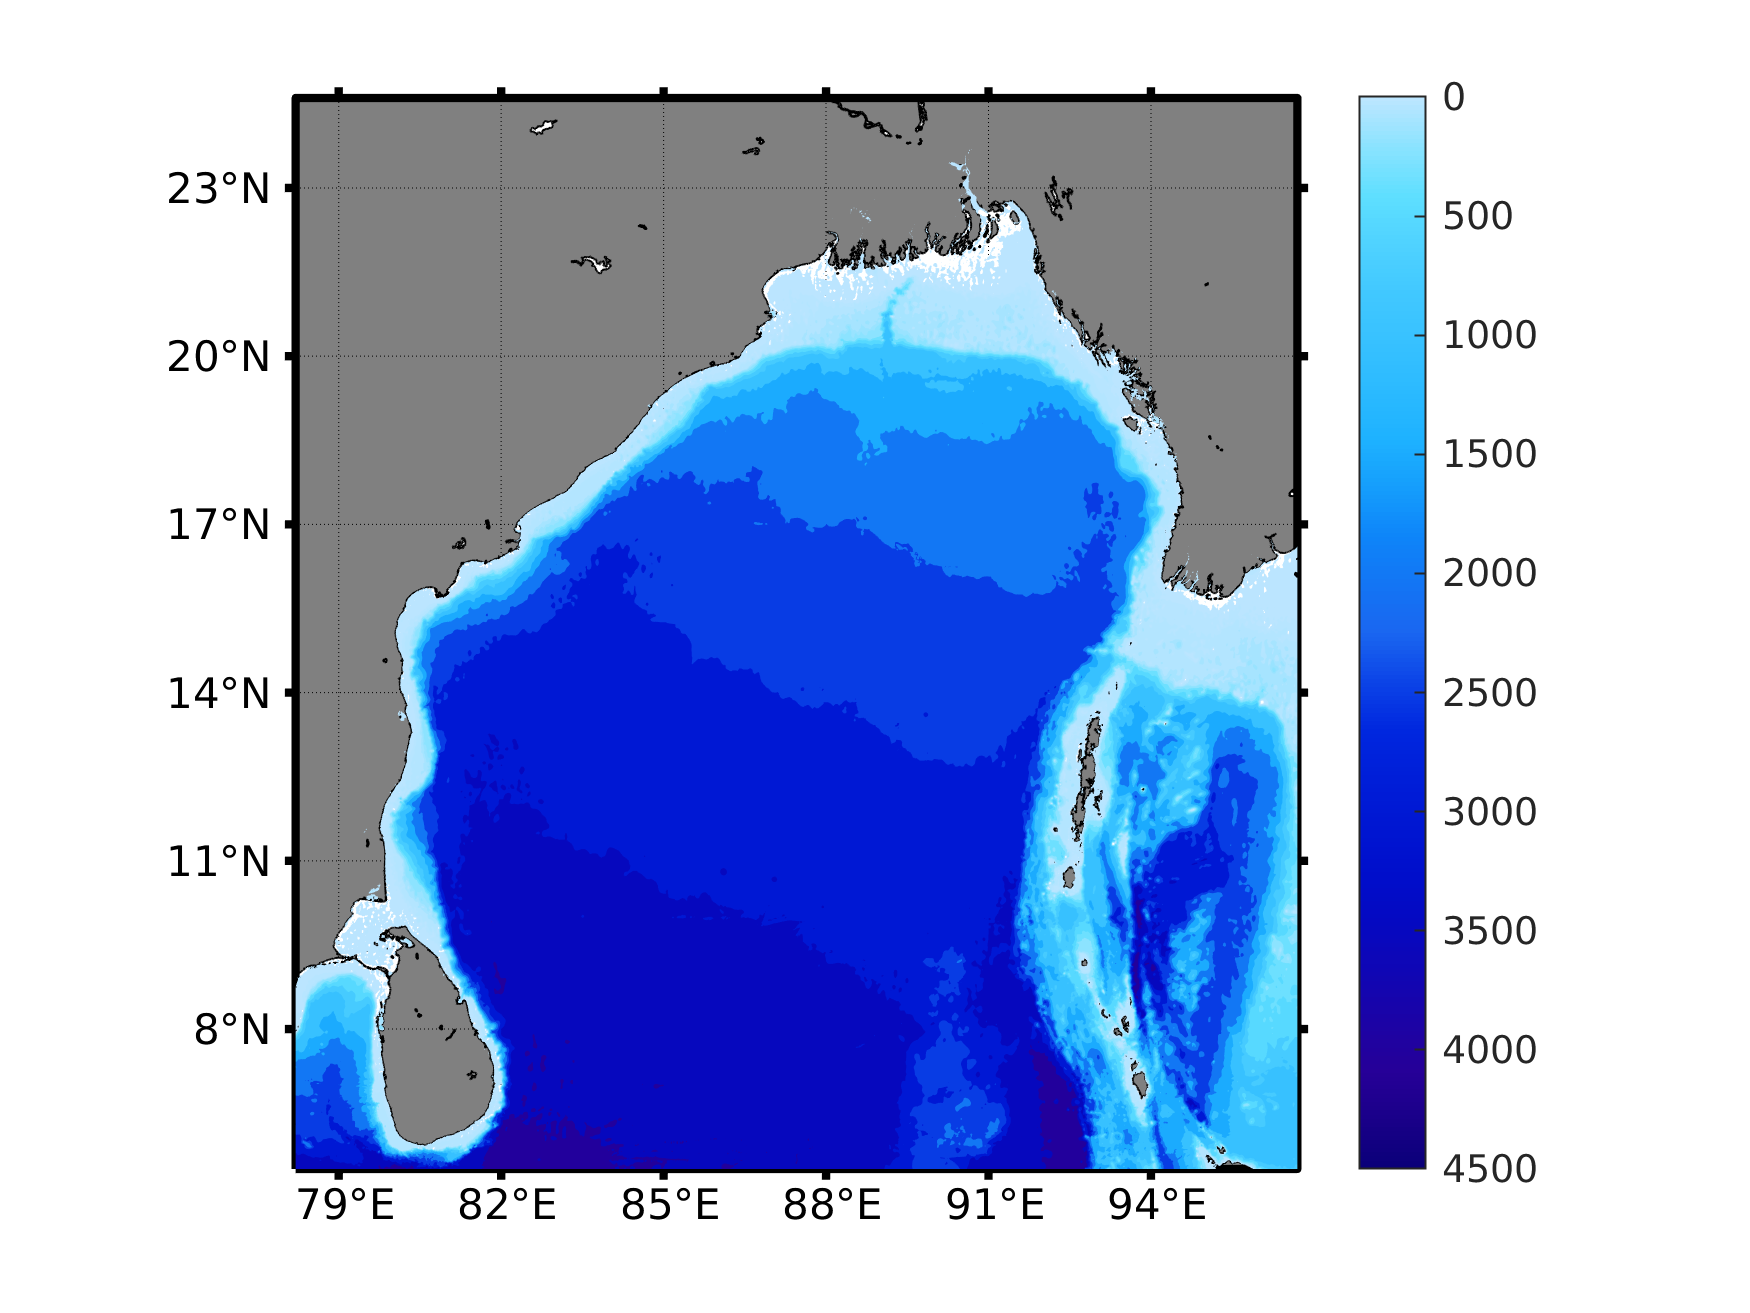
\includegraphics[width=7cm]{Topo_2}
		\captionsetup{labelformat=empty}
		\caption{Gambar 3.2. Data batimetri domain Teluk Benggala, dicuplik dari SRTM15+}
		\label{fig:domain_1}
	\end{figure}
\end{frame}

\subsection{Data Penelitian}
\begin{frame}
	\frametitle{Data Penelitian}
	\begin{figure}[H]
		\centering
		
\includegraphics[width=.5\textwidth]{logo_cmmes.png}
		\\[\smallskipamount]
		
\includegraphics[width=.24\textwidth]{logo_ncep.jpeg}
		\captionsetup{labelformat=empty}
		\caption{Gambar 3.4. Data penelitian}
		\label{fig:data}
		\tiny
		Data yang digunakan adalah data arus permukaan, serta data temperatur dari NEMO (resolusi spasial 5 mnt) dan data meteorologi (2m air temperature, 2m specific
		humidity, convective precipitation rate, sea level pressure, wind stress U, dan wind
		stress V) dari NCEP/NCAR selama 22 tahun dari tahun 2000 - 2021. 
	\end{figure}
\end{frame}

\subsection{Prosedur Penelitian}
\begin{frame}
	\frametitle{Prosedur Penelitian}
		\begin{figure}[H]
			\centering
			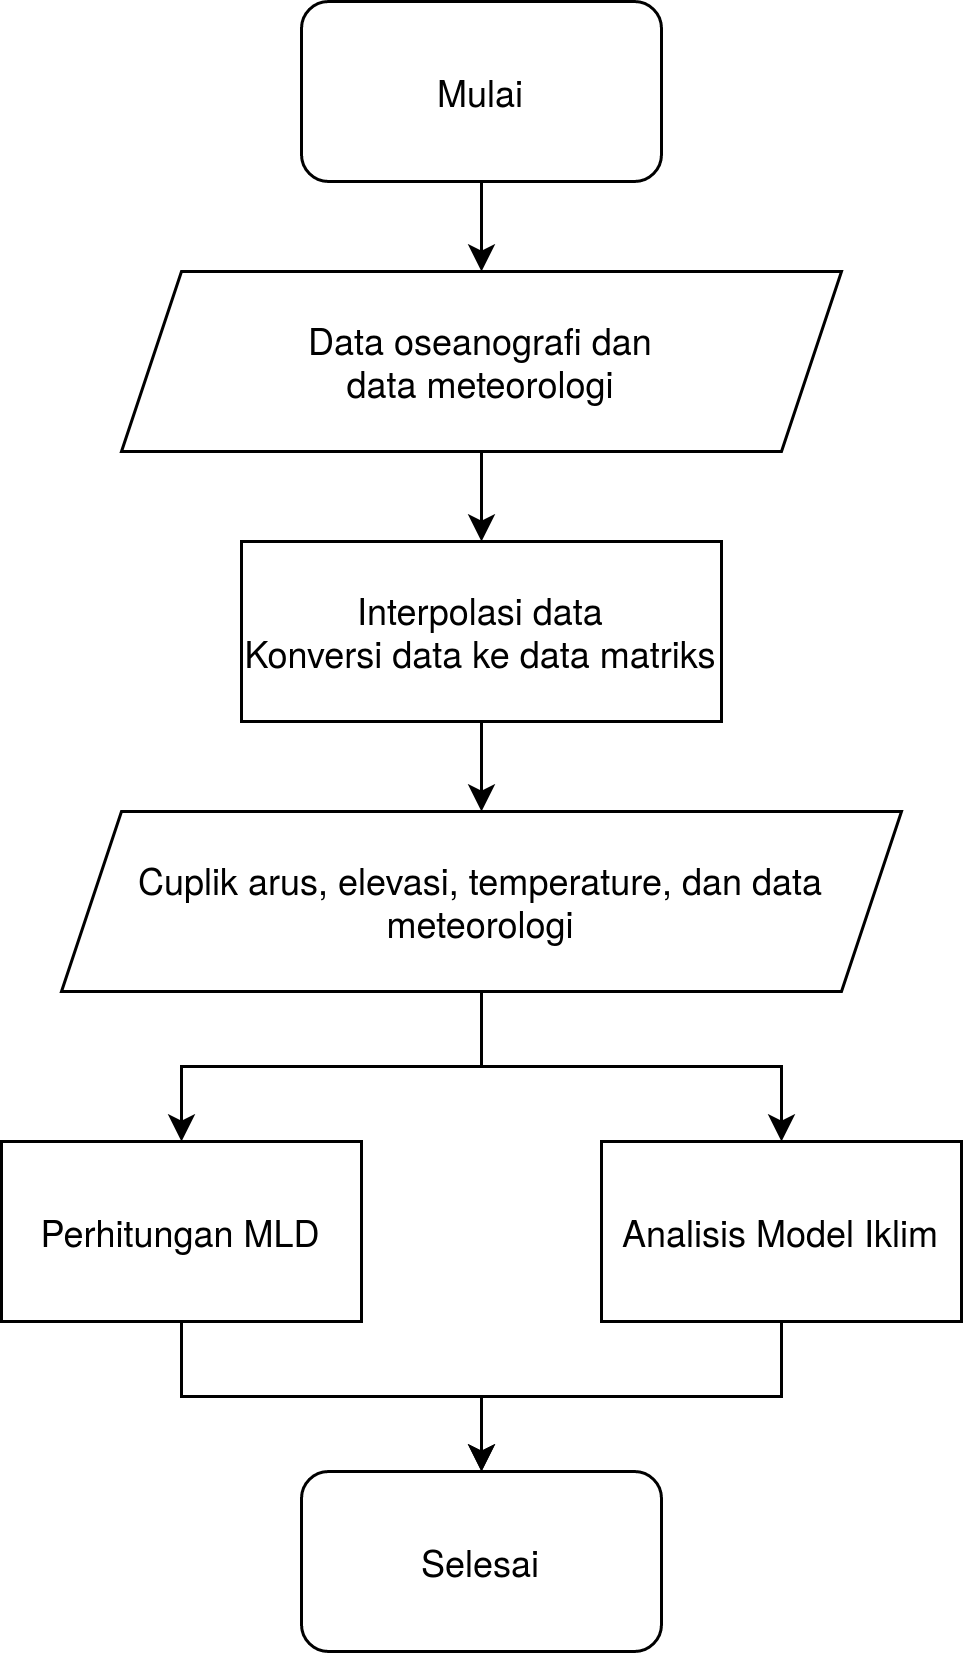
\includegraphics[width=4cm]{flowchart.png}
			\captionsetup{labelformat=empty}
			\caption{Gambar 3.5. Diagram alir penelitian}
			\label{fig:flowchart}
		\end{figure}
\end{frame}

\subsection{Jadwal Penelitian}
\begin{frame}
	\frametitle{Jadwal Penelitian}
		\begin{table}[htp]
			\centering
			\captionsetup{labelformat=empty}
			\caption{Tabel 3.1. Rencana jadwal pelaksanaan penelitian}
			\label{table:jadwal}
			\begin{tabular}{|c|c|ccccccc|}
				\hline
				\multirow{2}{*}{No.} & \multirow{2}{*}{Kegiatan} & \multicolumn{7}{c|}{Bulan}                                                                                                                            \\ \cline{3-9} 
				&                   & \multicolumn{1}{c|}{8} & \multicolumn{1}{c|}{9} & \multicolumn{1}{c|}{10} & \multicolumn{1}{c|}{11} & \multicolumn{1}{c|}{12} & \multicolumn{1}{c|}{1} &  2 \\ \hline 1
				& Studi literatur   & \multicolumn{1}{c|}{X} & \multicolumn{1}{c|}{X} & \multicolumn{1}{c|}{} & \multicolumn{1}{c|}{} & \multicolumn{1}{c|}{} & \multicolumn{1}{c|}{} &  \\ \hline 2
				& Seminar proposal    & \multicolumn{1}{c|}{X} & \multicolumn{1}{c|}{} & \multicolumn{1}{c|}{} & \multicolumn{1}{c|}{} & \multicolumn{1}{c|}{} & \multicolumn{1}{c|}{} &  \\ \hline 3
				& Pengumpulan data    & \multicolumn{1}{c|}{} & \multicolumn{1}{c|}{X} & \multicolumn{1}{c|}{} & \multicolumn{1}{c|}{} & \multicolumn{1}{c|}{} & \multicolumn{1}{c|}{} &  \\ \hline 4
				& Hasil dan analisis  & \multicolumn{1}{c|}{} & \multicolumn{1}{c|}{} & \multicolumn{1}{c|}{X} & \multicolumn{1}{c|}{X} & \multicolumn{1}{c|}{} & \multicolumn{1}{c|}{} &  \\ \hline 5
				& Seminar hasil       & \multicolumn{1}{c|}{} & \multicolumn{1}{c|}{} & \multicolumn{1}{c|}{} & \multicolumn{1}{c|}{} & \multicolumn{1}{c|}{X} & \multicolumn{1}{c|}{} &  \\ \hline 6
				& Ujian sidang        & \multicolumn{1}{c|}{} & \multicolumn{1}{c|}{} & \multicolumn{1}{c|}{} & \multicolumn{1}{c|}{} & \multicolumn{1}{c|}{} & \multicolumn{1}{c|}{X} &  \\ \hline 7
				& Publikasi           & \multicolumn{1}{c|}{} & \multicolumn{1}{c|}{} & \multicolumn{1}{c|}{} & \multicolumn{1}{c|}{} & \multicolumn{1}{c|}{} & \multicolumn{1}{c|}{X} & X  \\ \hline 
			\end{tabular}
		\end{table}
\end{frame}
\section{Output Proposal Tesis}
\begin{frame}[allowframebreaks]
	\frametitle{Output Proposal Tesis}
	Output dari proposal penelitian ini direncanakan dapat terpublikasi di beberapa konferensi dan jurnal berikut:
	\begin{itemize}
		\item Output konferensi AIC (Annual International Conference 2022), terindeks scopus.
		\item Output konferensi ICFAES (International Conference on Fisheries, Aquatic, and Environmental Sciences), terindeks scopus.
		\item Output jurnal JGR (Journal of Geophysical Research)
	\end{itemize}
	\begin{figure}[H]
		\centering
		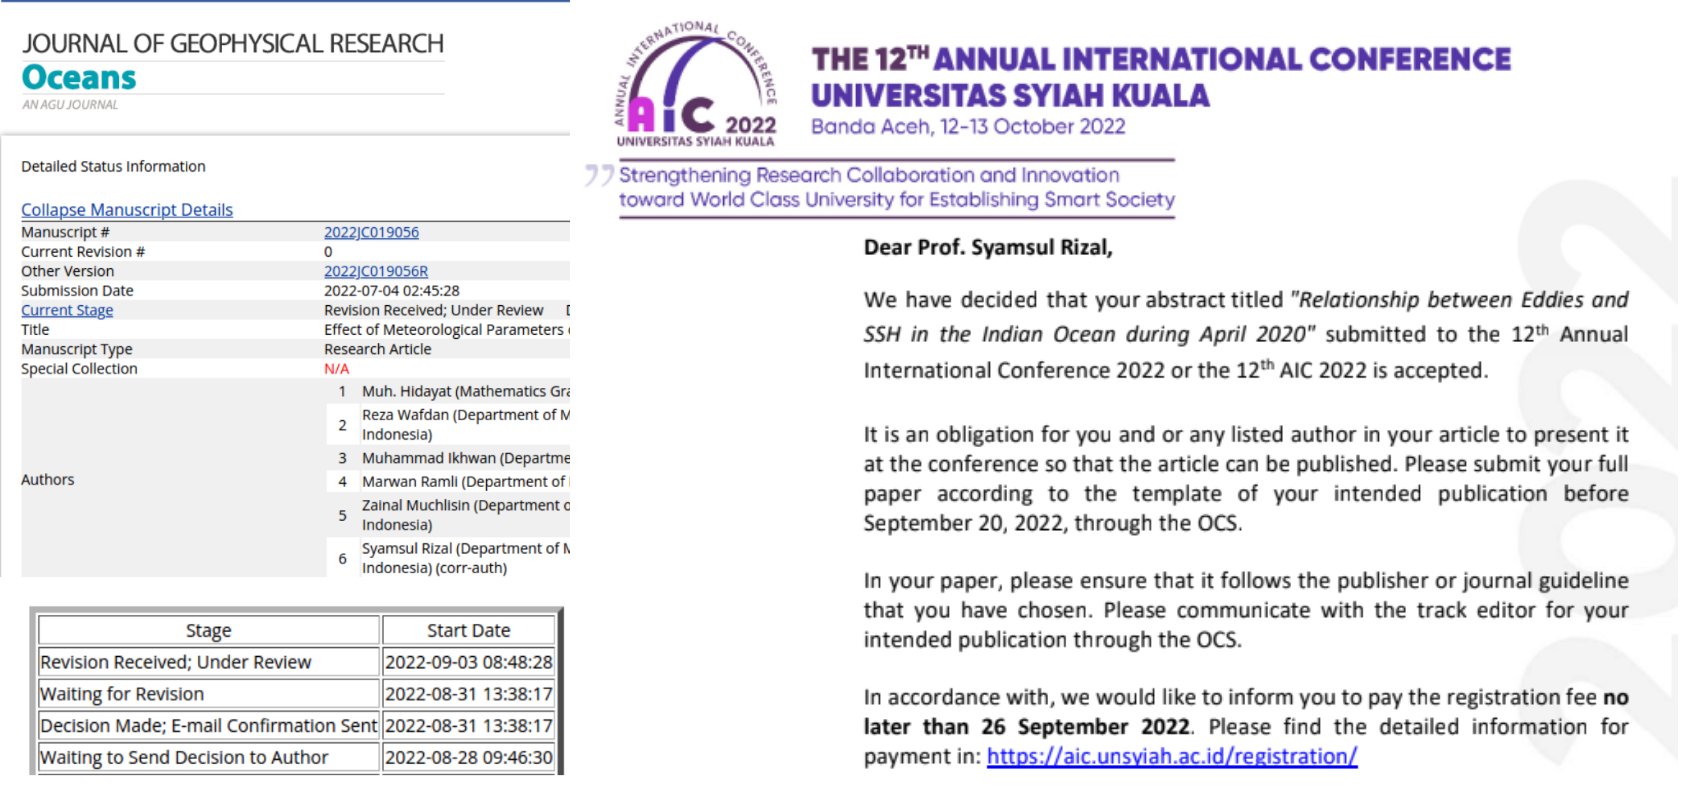
\includegraphics[width=10cm]{proof.png}
		\captionsetup{labelformat=empty}
	\end{figure}
\end{frame}
\ThankYouFrame

\end{document}